% !TEX TS-program = xelatex

\chapter{Symbolic modeling with Julia Plasm}
\label{chapt:5}

Symbolic modeling is a semantic approach to knowledge representation and processing. A  symbolic approach to design with the aim of representing information and computation uses names to define the meaning of represented knowledge explicitly. The geometric knowledge is described here by Julia's names, which are chosen suitably for functionals, functions, formal and actual parameters, and finally for objects, fields, classes, attributes, methods, relations, etc. In this chapter, we give many examples of high-level Plasm programming, from topological, linear, and affine operators, to geometric mapping of complexes and grids to generate linearized approximation of curved manifold of intrinsic dimensions 1, 2, and 3. i.e., depending on such number of parameters; say, curves, surfaces, thin, and bulk solids.



\section{ Primitive generators}\label{sect:5-1}

Here, we introduce both single objects and aggregates of cells, typically by grid and mesh generators, resulting in a single |Hpc| value after the evaluation.


\subsection*{Higher order and partial functions}\label{sect:5-1-0}

As we have already seen in Section \ref{}, Julia |Plasm| is higher-level since allows for function that take functions as argument and/or may return a function value.  All functions are objects of Julia |Function| type. As objects (holding a reference to the function code), can be assigned to a name (identifier).

\begin{definition}[Function order] The \emph{order} of an object of |Function| type is the number of applications to actual parameters needed to return the ultimate actual value,  not a partial function value (needing further parameters).
\end{definition}

\begin{coding}[\sf  INTERVALS(size::Numrber)(n::Int)] In this example we show a second-order function (requiring two applications) that generates a 1D complex made by |n| line segments of total given |size| length.
\begin{lstlisting}[language=JuliaLocal, style=julia, mathescape=true]
segments = INTERVALS(10::Number)(4::Int)		#=
Hpc(MatrixNd(2), Geometry([[0.0], [2.5], [5.0], [7.5], [10.0]], hulls=[[1, 2], [2, 3], [3, 4], [4, 5]]))		=#
\end{lstlisting}
Note that |segments| value is 1D since its 11 vertices have one coordinate. 
\end{coding}


\begin{coding}[\sf  QUOTE(measures::Array{Number})]\
The formal parameter is an array of signed numbers.
\begin{lstlisting}[language=JuliaLocal, style=julia, mathescape=true]
two_aligned_segments = QUOTE([1,-2.5,1])			#=
Hpc(MatrixNd(2), Geometry([[0.0], [1.0], [3.5], [4.5]], hulls=[[1, 2], [3, 4]]))	=#
\end{lstlisting}
Positive numbers denote solid intervals of a given size; negative numbers denote hollow space, i.e., displacement of following segments. Successive negative numbers are allowed.\end{coding}


\begin{coding}[\sf  Q(measure::Number)]\
The formal parameter is a signed number. 
\begin{lstlisting}[language=JuliaLocal, style=julia, mathescape=true]
segment = Q(10)
Hpc(MatrixNd(2), Geometry([[0.0], [10.0]], hulls=[[1, 2]]))
\end{lstlisting}
A single |segment| of given size.
\end{coding}


\subsection*{Single convex cell}\label{sect:5-1-1}

Julia |Plasm| contains a great library of generator functions of very simple objects made by a single convex cell, and completely specified by its set of vertices only. 
Few examples follow; Other examples can be extracted or generated by the user looking at file |src/fenvs.jl|, including the Platonic solids. The multidimensional $d$-permutaheron is generated in Coding \ref{4-2-permutahedron}. 

\begin{coding}[\sf  CUBOID(size)]\
Multidimensional cuboid with |sizes::Vector{Number}|.
\begin{lstlisting}[language=JuliaLocal, style=julia, mathescape=true]
CUBOID([1])			#=
Hpc(MatrixNd(2), Hpc(MatrixNd(2), Geometry([[0.0], [1.0]], hulls=[[1, 2]]))) =#

CUBOID([1,2])			#=
Hpc(MatrixNd([[1.0, 0.0, 0.0], [0.0, 1.0, 0.0], [0.0, 0.0, 2.0]]), Hpc(MatrixNd(3), Geometry([[0.0, 0.0], [1.0, 0.0], [1.0, 1.0], [0.0, 1.0]], hulls=[[1, 2, 3, 4]]))) =#

CUBOID([1,2,3])			#=
Hpc(MatrixNd([[1.0, 0.0, 0.0, 0.0], [0.0, 1.0, 0.0, 0.0], [0.0, 0.0, 2.0, 0.0], [0.0, 0.0, 0.0, 3.0]]), Hpc(MatrixNd(4), Geometry([[0.0, 0.0, 0.0], [1.0, 0.0, 0.0], [0.0, 1.0, 0.0], [1.0, 1.0, 0.0], [0.0, 0.0, 1.0], [1.0, 0.0, 1.0], [0.0, 1.0, 1.0], [1.0, 1.0, 1.0]], hulls=[[1, 2, 3, 4, 5, 6, 7, 8]]))) =#

CUBOID([1,2,3,4])			#=
Hpc(MatrixNd([[1.0, 0.0, 0.0, 0.0, 0.0], [0.0, 1.0, 0.0, 0.0, 0.0], [0.0, 0.0, 2.0, 0.0, 0.0], [0.0, 0.0, 0.0, 3.0, 0.0], [0.0, 0.0, 0.0, 0.0, 4.0]]), Hpc(MatrixNd(5), Geometry([[0.0, 0.0, 0.0, 0.0], [1.0, 0.0, 0.0, 0.0], [0.0, 1.0, 0.0, 0.0], [1.0, 1.0, 0.0, 0.0], [0.0, 0.0, 1.0, 0.0], [1.0, 0.0, 1.0, 0.0], [0.0, 1.0, 1.0, 0.0], [1.0, 1.0, 1.0, 0.0], [0.0, 0.0, 0.0, 1.0], [1.0, 0.0, 0.0, 1.0], [0.0, 1.0, 0.0, 1.0], [1.0, 1.0, 0.0, 1.0], [0.0, 0.0, 1.0, 1.0], [1.0, 0.0, 1.0, 1.0], [0.0, 1.0, 1.0, 1.0], [1.0, 1.0, 1.0, 1.0]], hulls=[[1, 2, 3, 4, 5, 6, 7, 8, 9, 10, 11, 12, 13, 14, 15, 16]]))) =#
\end{lstlisting}
Cuboids of given sizes. Of course, the unit hypercube in $\E^6$ has |size = [1,1,1,1,1,1]|. 
\end{coding}

The |Plasm| coding of the “icosphere”, polyhedral approximation of the 2-sphere obtained by subdividing the |ICOSAHEDRON()| surface is given here, starting from the Platonic solid. The generation method is extremely simple. We obtain the vertices at step $i+1$ by adding to the vertices at step $i$ those obtained by subdivision of all edges. Ma make use of theHpc structure and the Lar structure.


\begin{coding}[\sf  ICOSPHERE(seed::Hpc)::Hpc]\
First we generate the cell complex of the input |obj| using the |LAR| combinator, then for each edge we compute the mean point, then we aggregate to the old vertices the new ones, scaled by the factor |r1/s1| built with the distance from |[0,0,0]| center of both models.
\begin{lstlisting}[language=JuliaLocal, style=julia, mathescape=true]
function ICOSPHERE(obj::Hpc)::Hpc
 W  = LAR(obj).V
 EV = LAR(obj).C[:EV]
 W  = [W[:,k] for k=1:size(W,2)]
 V  = [(W[v1]+W[v2])./2 for (v1,v2) in EV]
 r1 = sqrt(sum(W[1].^2))
 s1 = sqrt(sum(V[1].^2))
 CONVEXHULL([W; V*(r1/s1)]);
end
\end{lstlisting}
Finally, the |[W; V*(r1/s1)]::Vector{Vector{Float64}}| made by old vertices and by new scaled ones is given to the operator |CONVEXHULL| that transforms such a |Vector| of point (|Vector{Float64}|) in their geometric \emph{convex hull}.
Just remember that such polyhedra are convex sets, hence they have a \emph{single} (convex) cell. \begin{lstlisting}[language=JuliaLocal, style=julia, mathescape=true]
out0 = ICOSAHEDRON(); VIEW(out0)
out1 = ICOSPHERE(out0); VIEW(out1)
out2 = ICOSPHERE(out1); VIEW(out2)
out3 = ICOSPHERE(out2); VIEW(out3)
...		
\end{lstlisting}
Successive approximations of icosphere with 12, 42, 162, 600, etc., vertices.
Let’s remark the extreme simplicity of such polyhedral generations.
\end{coding}

\begin{figure}[htbp] %  figure placement: here, top, bottom, or page
 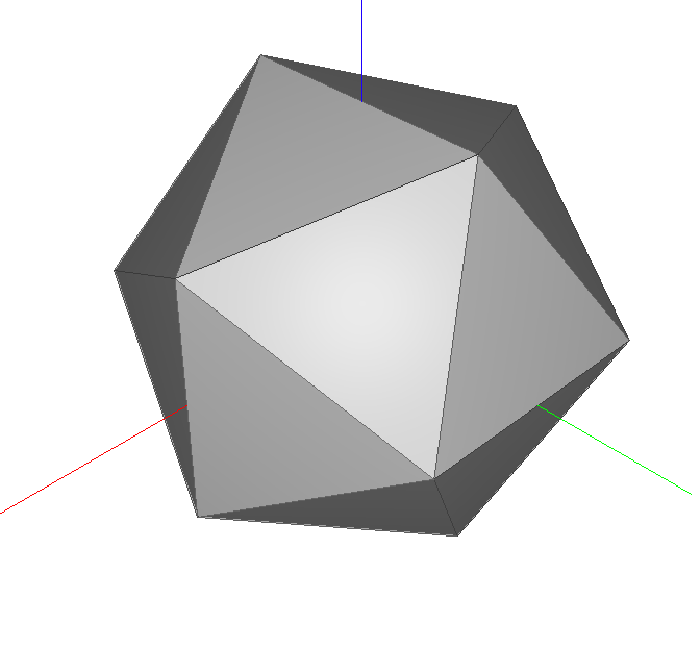
\includegraphics[width=0.34\linewidth]{chapter-05/figs/icosphere0}%
 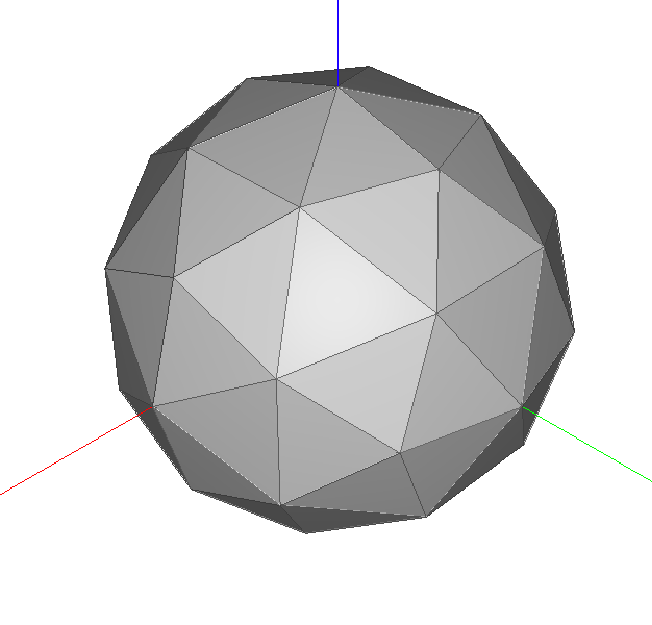
\includegraphics[width=0.33\linewidth]{chapter-05/figs/icosphere1}%
 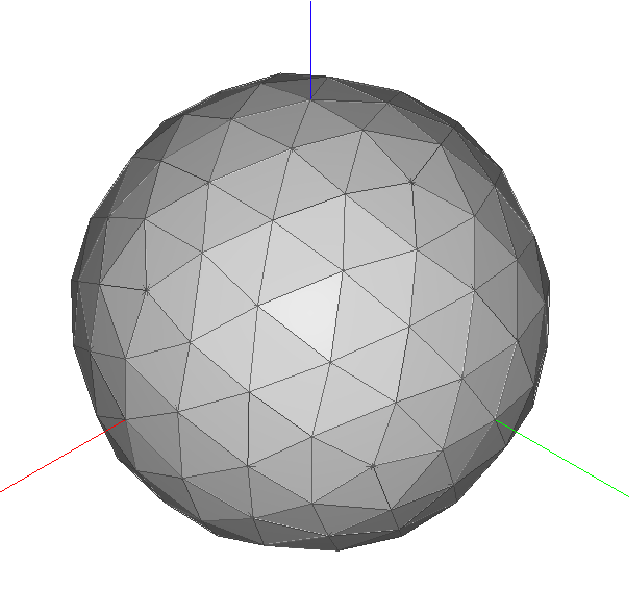
\includegraphics[width=0.325\linewidth]{chapter-05/figs/icosphere2}%
\hfill
\caption{(a) Icosahedron; (b) icosphere with 42 vertices; (c)  icosphere with 162 vertices. }
\label{5:icospheres}
\end{figure}



\subsection*{Multiple cell objects}\label{sect:5-1-1}


The functions |INTERVALS| or |QUOTE| may be used to create many types and patterns of grid geometries.

\begin{script}[Building frame]\
First we give the main dataset of a building frame, by “quoting” the side measures of 2D design plan:
\begin{lstlisting}[language=JuliaLocal, style=julia, mathescape=true]
# Longitudinal trusses
Y = QUOTE([0.3, -6, 0.3, -6, 0.3])
# transverse beams
X = QUOTE([0.3, -3, 0.3, -4.2, 0.3, -3, 0.3])
# vertical measurements
Z = QUOTE([3,0.3])
\end{lstlisting}
Then, an alternate set of |INTERVALS| vector parameters are generated by Julia broadcast |.*| of the scalar |-1|, in order to invert all the signs.
\begin{lstlisting}[language=JuliaLocal, style=julia, mathescape=true]
X1 = QUOTE([0.3, -3, 0.3, -4.2, 0.3, -3, 0.3].* -1)
Y1 = QUOTE([0.3, -6, 0.3, -6, 0.3].*-1)
Z1 = QUOTE([3,-0.3].*-1)
\end{lstlisting}
Below, the 3D |frame| subsystems are generated. They are the $C_3$ basis of a local cellular complex. Note the variation pattern at |trusses1|.
\begin{lstlisting}[language=JuliaLocal, style=julia, mathescape=true]
# Cartesian product
pillars = COLOR(RED)(X*Y*Z);
trusses = COLOR(YELLOW)(X*Y1*Z1);
trusses1 = COLOR(YELLOW)(X1*Y*QUOTE([-2.7,0.6]));
floorslab = COLOR(GREEN)(X1*Y1*Z1);
\end{lstlisting}
Finally, the sub-complexes of 3D cells are aggregated in a single |Plasm| complex using the |STRUCT| combinator discussed in the next session. Let us note that in this example all the aggregated models live in the same reference frame.
\begin{lstlisting}[language=JuliaLocal, style=julia, mathescape=true]
frame = STRUCT(pillars, trusses, trusses1, floorslab);
VIEW(frame, Dict("background_color"=>WHITE))
\end{lstlisting}
\end{script}


\begin{figure}[htbp] %  figure placement: here, top, bottom, or page
 \sidecaption[t]
 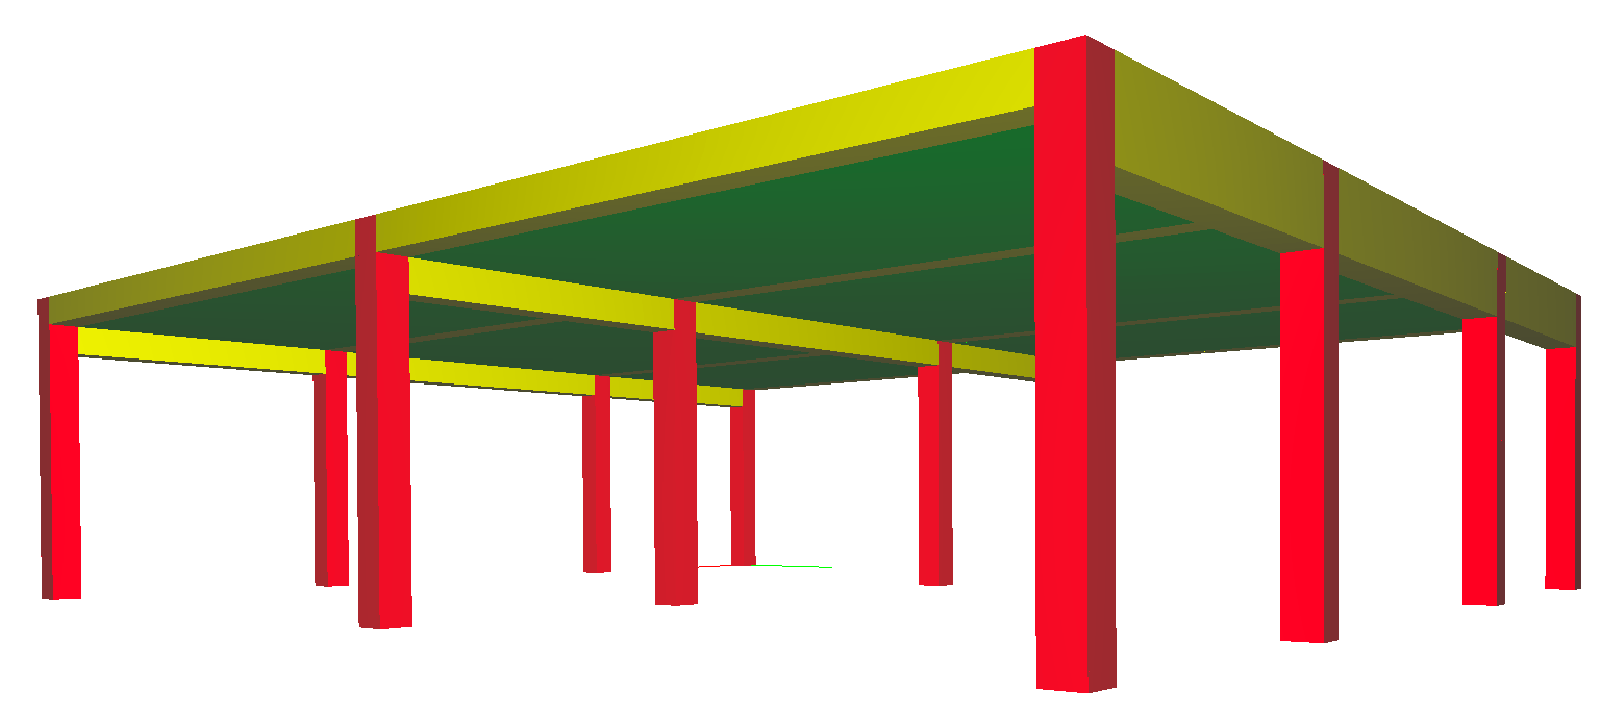
\includegraphics[width=\linewidth]{chapter-05/figs/frame1} 
 \caption{\sf frame = STRUCT(pillars, trusses, trusses1, floorslab);}.}
 \label{fig:example}
\end{figure}
\subsection*{Assembly combinator {\sf STRUCT}}\label{sect:5-1-1}

We have already come across the |STRUCT| function, one of more important |Plasm| operators. In particular, we already know that |STRUCT| is used to assembly geometric objects into a single object. In Julia |Plasm| both the input and the output objects are of recursive |Hpc| type.

In geometric modeling of complex assemblies the geometric and graphics
programmer makes wide use of the \emph{hierarchical scene
graphs}~\cite{Wernecke:94:TIM,Sowizral:2000:J3DAPI} or hierarchical
structures~\cite{Gaskins92}, where sub-assemblies are defined in \emph{local}
coordinates, and are transformed into the coordinate frame of the
output assembly by explicitly using proper coordinate
transformations.  

It is worth noting that such “modeling transformations" --- as they are called in graphical systems --- are left entirely to programmer's responsibility.  


\begin{figure}[htbp] %  figure placement: here, top, bottom, or page
 \sidecaption[t]
 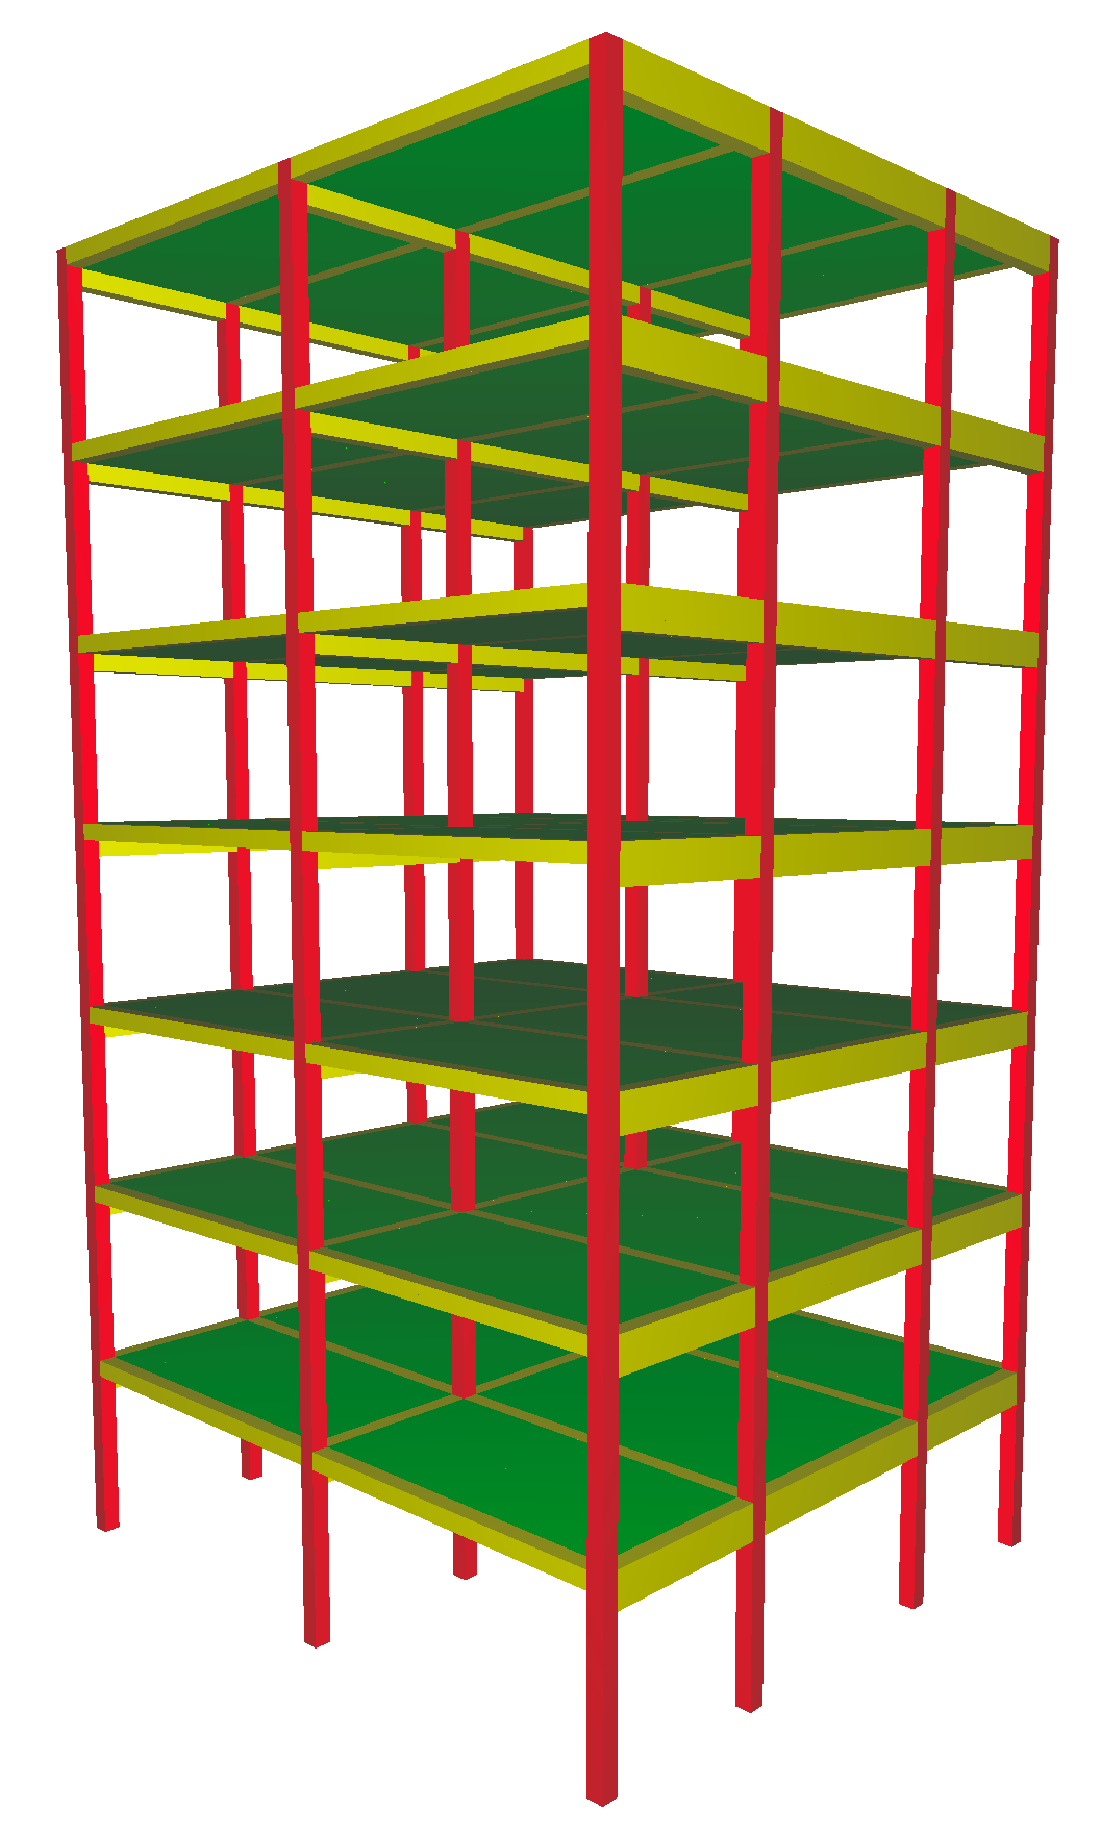
\includegraphics[width=0.6\linewidth]{chapter-05/figs/skeleton1} 
 \caption{\sf skeleton = STRUCT(NN(7)([frame, T(3)(3.3)])));}.}
 \label{fig:5:1:skeleton}
\end{figure}

\begin{coding}[Building skeleton]\label{5:1:skeleton}
We assemble here a building skeleton model, by creating a |STRUCT| assembly generated by |n=7| instances of the Julia |Vector| made by the |Hpc| value |frame| and by the |MatrixNd| value |T(3)(3.3)| producing a translation in $z$ direction.
\begin{lstlisting}[language=JuliaLocal, style=julia, mathescape=true]
skeleton = STRUCT(NN(7)([frame, T(3)(3.3)]));
VIEW(skeleton, Dict("background_color"=>WHITE)
\end{lstlisting}
\end{coding}

Here the |STRUCT| semantics is very clear: the evaluated subexpression |NN(7)([frame, T(3)(3.3)])| is an array of type |Vector{Union{Hpc, MatrixNd}}| and contain 14 item with alternating types.  When |STRUCT| is evaluted on this vector, an |Hpc| node is generated, whose |MatrixNd| field contains a $4\times 4$ identity matrix, and the |childs| vector contains the reference to the first item of 


\subsection*{Alignment aggregators {\sf TOP, BOTTOM, LEFT, RIGTH}}\label{sect:5-1-1}


In the present section we discuss some simplified assembly operators, where the
coordinate transformations are computed automatically by the language.

|Plasm| has some predefined binary functions used to locate two complexes with respect each other.  In particular,
the second argument of such functions will be positioned either
|TOP| the first one, or |ABOVE|, or |LEFT|, or
|RIGHT|, or |UP|, or |DOWN|, respectively,
according to the alignment semantics given below.

Such relative positioning allows
for an easy construction of complex assemblies, without taking into account the local coordinate frames where the
sub-assemblies are defined.  In this way we avoid applying affine transformations as it is
conversely needed in hierarchical scene graphs.

\begin{coding}[alternate method for vertical aggregation]\
\begin{lstlisting}[language=JuliaLocal, style=julia, mathescape=true]
multifloor(model,n) = STRUCT(INSR(TOP)(N(n+1)(model))) #=
multifloor (generic function with 1 method)		  	 =#
VIEW(multifloor(frame,7))
\end{lstlisting}
The object generated here is equal to the |skeleton| model of Figure \ref{fig:5:1:skeleton}. 
\end{coding}

|TOP| is a binary function of two |Hpc| models that creates their vertical aggregation.
Any binary function is transformed in $n$-ary by the second order operator |INSR| (for \emph{insert right}). |INSR| is applied first to the operator argument to make $n$-ary, then to the list of objects the operator apply to.

|N(n)(value::Any)| is a |Plasm| function called $\#$ in classic |PLaSM|, that returns a list of |n| instances of |value|. 

\begin{definition}[Primitive {\sf ALIGN} function.]
Every pair of polyhedral complexes may be aligned along any given subset of coordinates by using the primitive binary function |ALIGN|. Such a second-order operator must be applied to a sequence of triples which define a specialized behavior for each affected coordinate.
\end{definition}

Each alignment directive along a coordinate must belong to the set
\[
[1,n] \times \{ |MIN,MED,MAX,K($\alpha$)|\} 
\times \{ |MIN,MED,MAX,K($\alpha$})|\}
\]
where |$\alpha$::Number|, used to align on a given coordinate. The resulting specialized operator is then applied to a pair of |Hpc| values, and returns a single |Hpc|.  Use examples following the |ALIGN| combinator for other operators' definitions.
\begin{lstlisting}[language=JuliaLocal, style=julia, mathescape=true]
TOP = ALIGN([[3, MAX, MIN], [1, MED, MED], [2, MED, MED]])
BOTTOM = ALIGN([[3, MIN, MAX], [1, MED, MED], [2, MED, MED]])
LEFT = ALIGN([[1, MIN, MAX], [3, MIN, MIN]])
RIGHT = ALIGN([[1, MAX, MIN], [3, MIN, MIN]])
UP = ALIGN([[2, MAX, MIN], [3, MIN, MIN]])
DOWN = ALIGN([[2, MIN, MAX], [3, MIN, MIN]])
# 294 (generic function with 1 method)
\end{lstlisting}


\begin{figure}[htbp] %  figure placement: here, top, bottom, or page
 \sidecaption[t]
 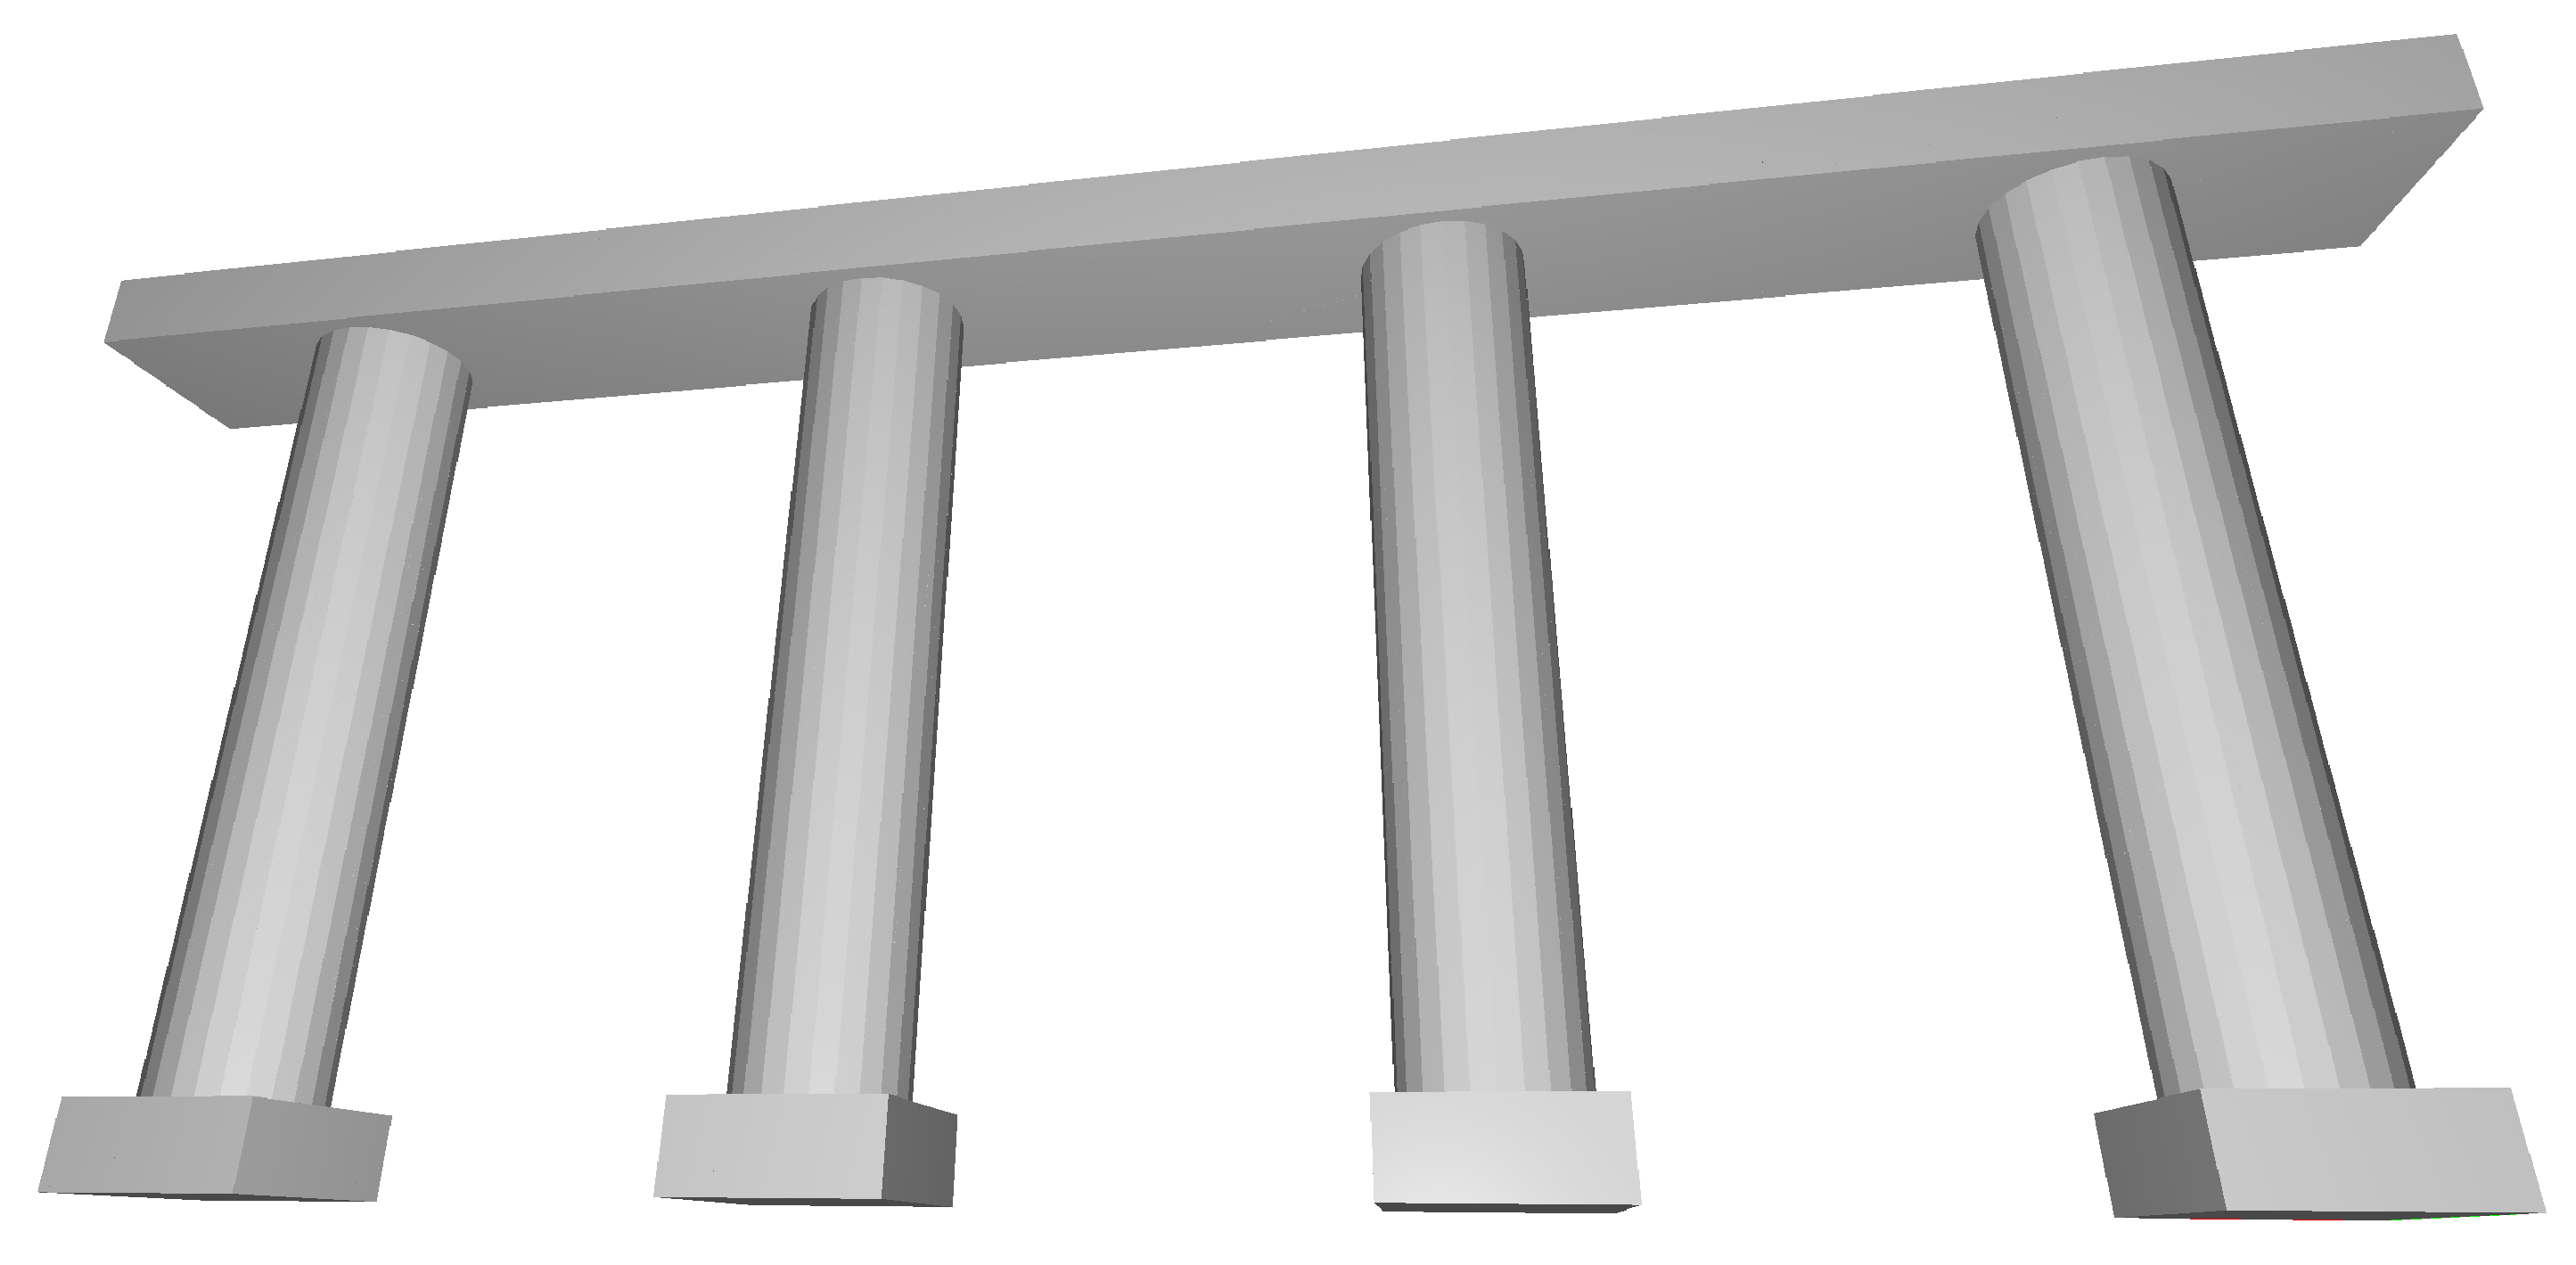
\includegraphics[width=\linewidth]{chapter-05/figs/fourcolumns} 
 \caption{\sf skeleton = STRUCT(NN(7)([frame, T(3)(3.3)])));}.}
 \label{fig:5:1:fourcolumns}
\end{figure}

\begin{coding}\
A very simplified view of a column is built here, to show the use of the |INSR(TOP)| and |INSR(RIGHT)| functions applied to a list of geometric object, each given in its local coordinate system:
\begin{lstlisting}[language=JuliaLocal, style=julia, mathescape=true]
function Column(r,h)
 basis = CUBOID([ 2*r*1.2, 2*r*1.2, h/12.0 ]) 
 trunk = CYLINDER([ r, (10.0/12.0)*h ])(12)
 capital = CUBOID([ 2*r*1.2, 2*r*1.2, h/12.0 ])
 beam = S(1)(3)(capital) 
 return INSR(TOP)([basis,trunk,capital,beam])
end
# Column (generic function with 2 methods)
\end{lstlisting}

\begin{lstlisting}[language=JuliaLocal, style=julia, mathescape=true]
function ColRow(N,r,h)
 col = Column(r,h)
 columnlist = [col for k in 1:N+1]
 return INSR(RIGHT)(columnlist)
end
# ColRow (generic function with 2 methods)
\end{lstlisting}

\begin{lstlisting}[language=JuliaLocal, style=julia, mathescape=true]
VIEW(ColRow(4,1.,12.), Dict( => WHITE))
\end{lstlisting}
The generated model is displayed in Figure \ref{}
\end{coding}



\begin{figure}
\begin{minipage}[t]{0.571\linewidth}
	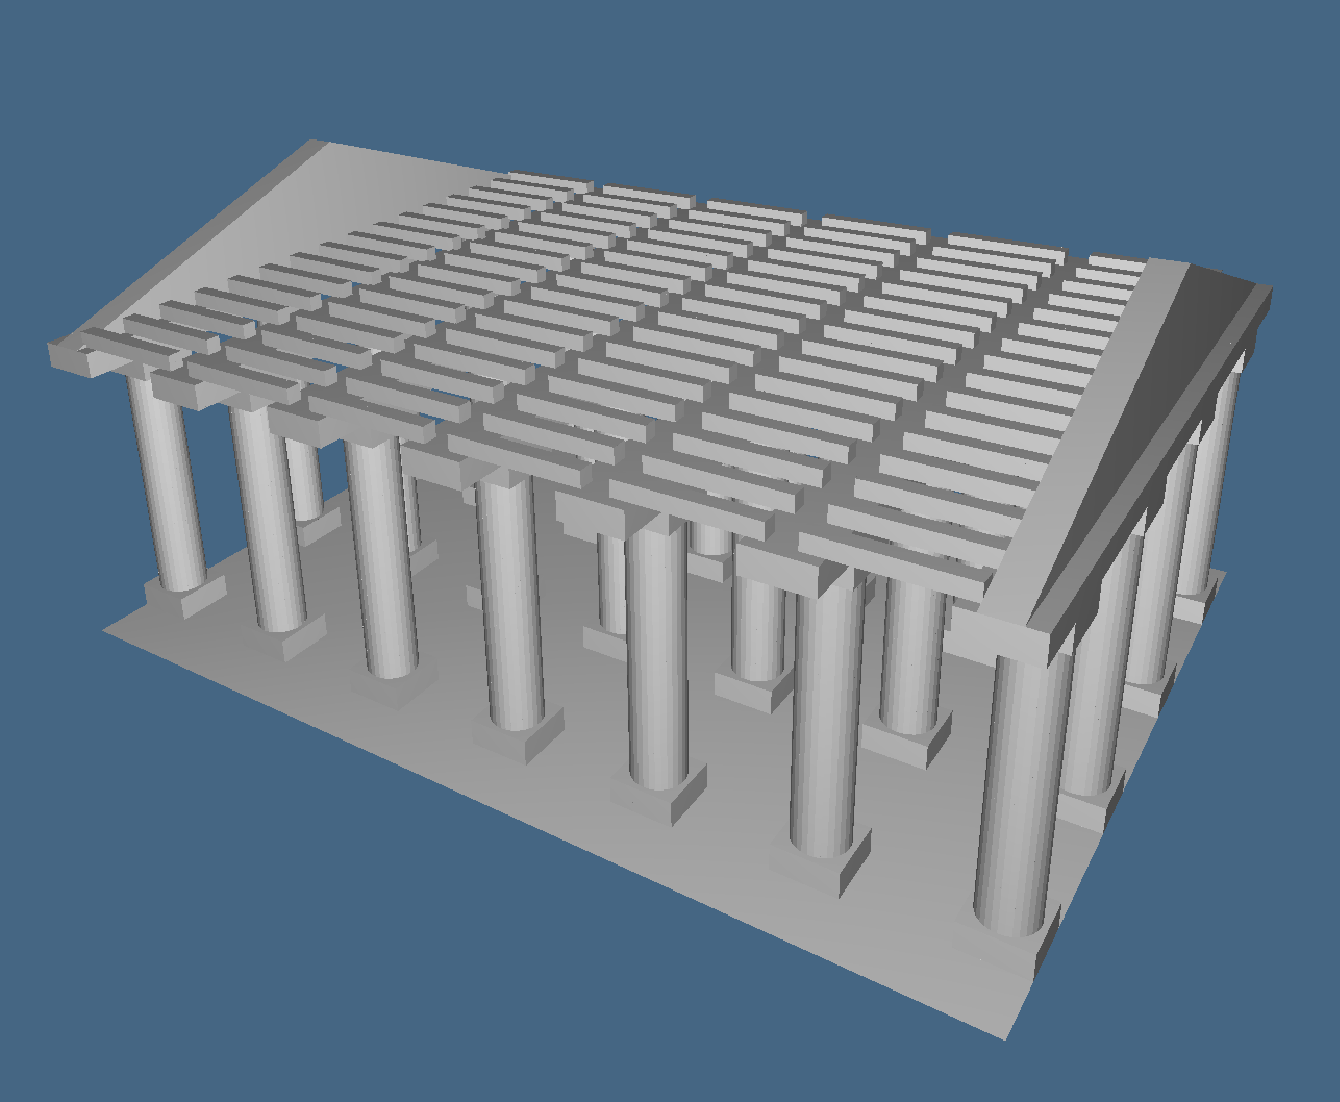
\includegraphics[width=\linewidth]{chapter-05/figs/temple-01}%

		\vspace{-1mm}
	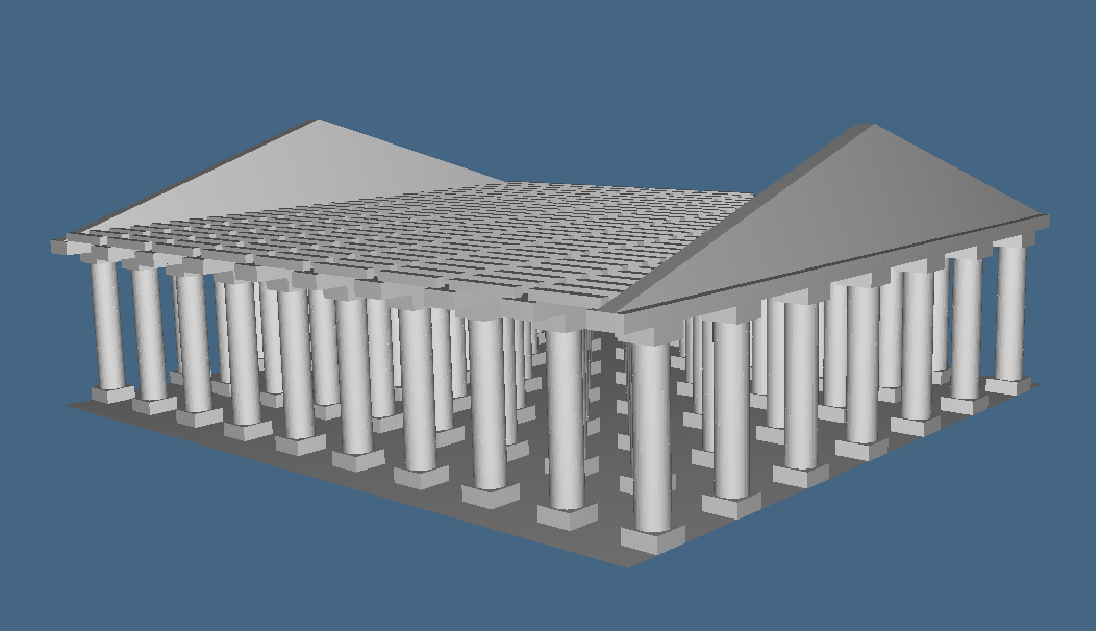
\includegraphics[width=\linewidth]{chapter-05/figs/temple-02}
	%\label{fig:example}
\end{minipage}%
\begin{minipage}[t]{0.429\linewidth}
	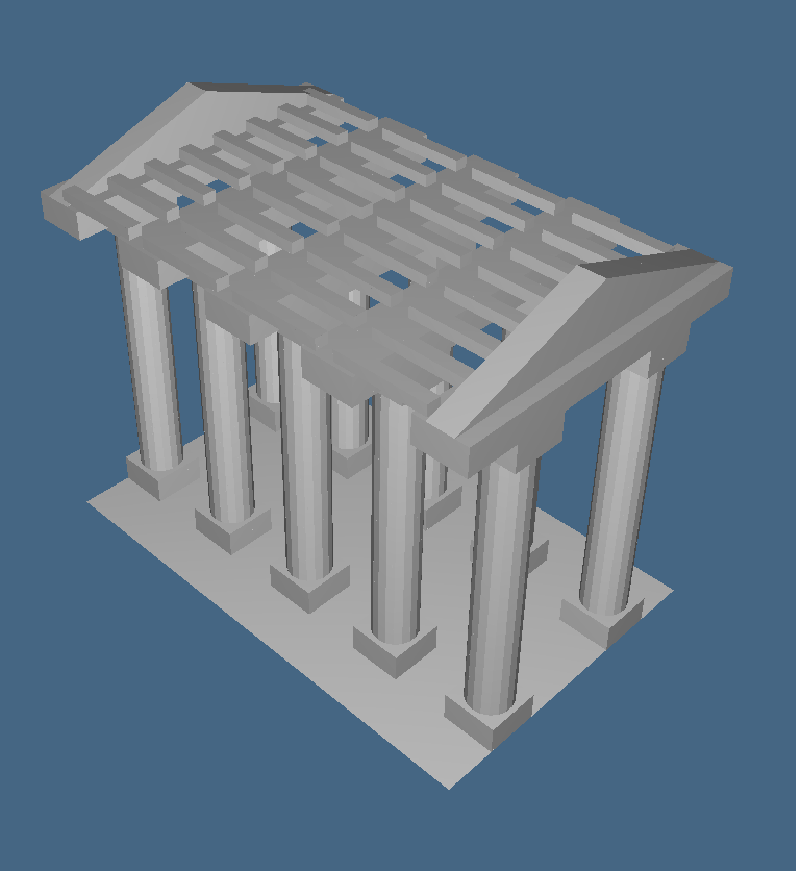
\includegraphics[width=\linewidth]{chapter-05/figs/temple-03}
\caption{A fully parameterized {\sf Temple()} function, where several parameters are linked to each other by algebraic equations. Let’s note the number of side and front columns, and their relations with column height and gable width. The whole function code is about 15 rows.}
\end{minipage}
\end{figure}




\section{ Plasm topological operators}\label{sect:5-2}

For the sake of simplicity, we start here our presentation of programming through  topological operators by discussing with one of simplest example models, the |Lar| numbered version of the 3-cube of side 1. Both the vector font of text and its integrated display with the object are by |Plasm| package.  Such integration with text was of invaluable utility in algorithm development.

First, in this model we have a 3D chain complex (see section~\ref{sect:3-3-2}) with 
one 3-cell, 6 faces (2-cells |FV|), 12 edges (1-cells |EV|), and 8 vertices (0-cells |V|).

\begin{figure}[htbp] %  figure placement: here, top, bottom, or page
 \sidecaption[t]
 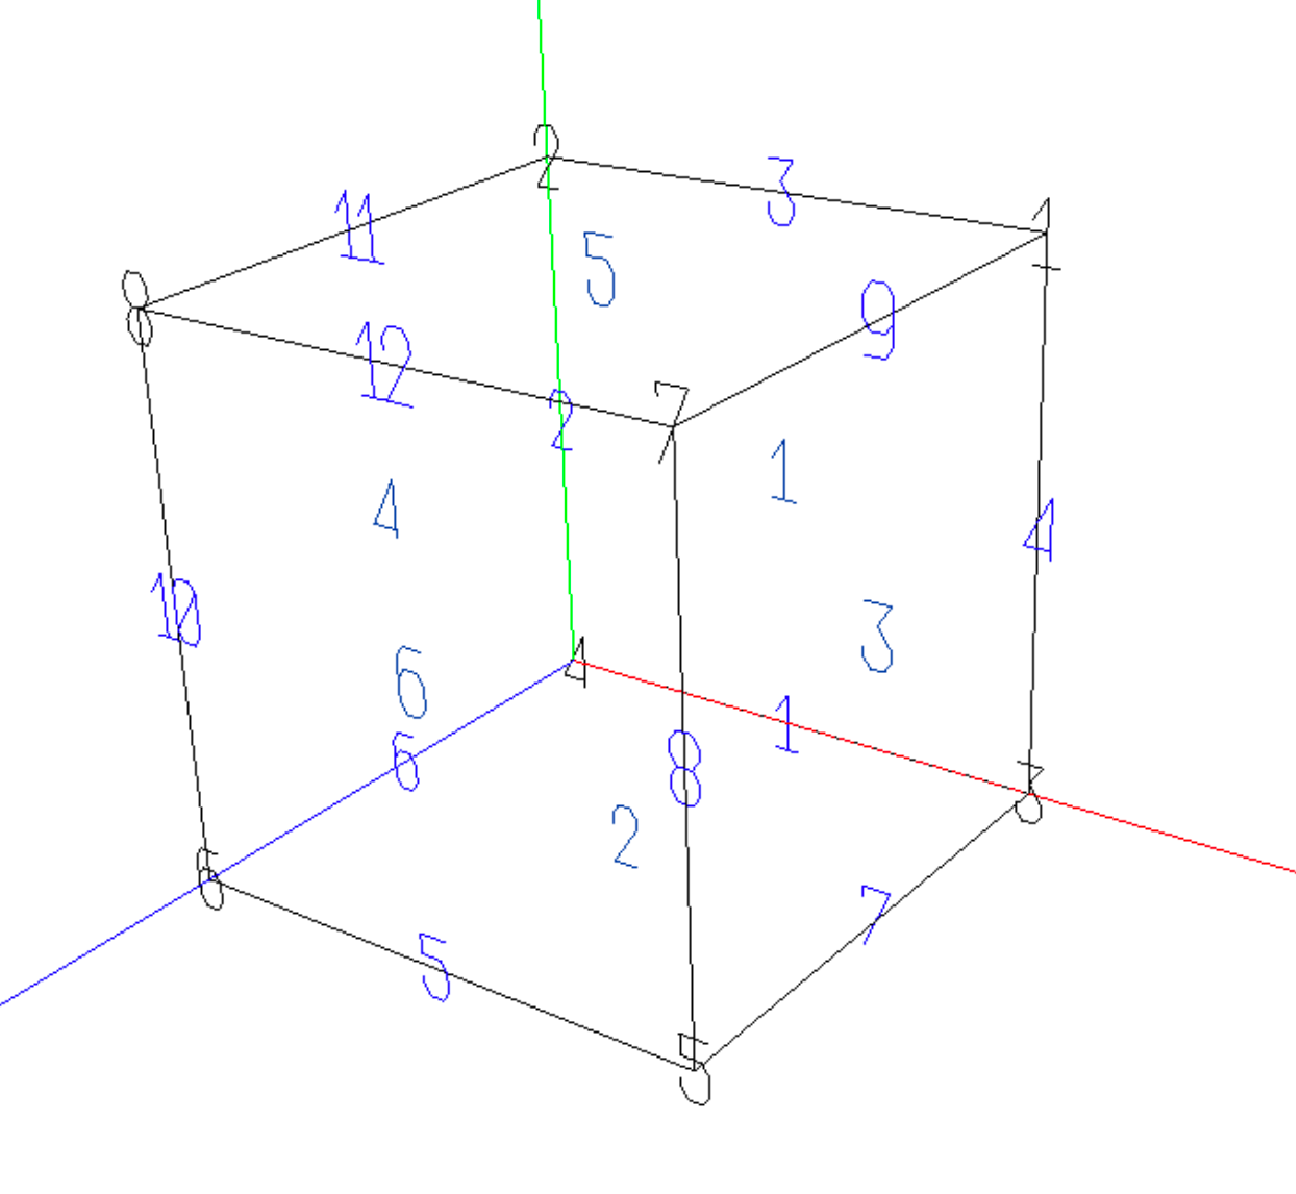
\includegraphics[width=0.5\linewidth]{chapter-05/figs/cube} 
 \caption{The numbered unit 3-cube cellular complex. 
 The ordinal numbers  for vertices, edges and faces are set at the middle of each 1-, 2-, and 3-cell. Note that the indexes have lexicographic and not geometric order (say, clockwise or counterclockwise), but this is not a constraint. }
 \label{fig:5:1:cube}
\end{figure}
The reader is instructed to check for comparison the following dataset with the Figure~\ref{fig:5:1:cube}. In general, the cell indices are unordered.
\begin{lstlisting}[language=JuliaLocal, style=julia, mathescape=true]
LAR(CUBE(1))		#=
Lar(3, 3, 8, [1.0 0.0 … 1.0 0.0; 1.0 1.0 … 1.0 1.0; 0.0 0.0 … 1.0 1.0], Dict{Symbol, AbstractArray}(:CV => [[1, 2, 3, 4, 5, 6, 7, 8]], :FV => [[1, 2, 3, 4], [3, 4, 5, 6], [1, 3, 5, 7], [2, 4, 6, 8], [1, 2, 7, 8], [5, 6, 7, 8]], :EV => [[3, 4], [2, 4], [1, 2], [1, 3], [5, 6], [4, 6], [3, 5], [5, 7], [1, 7], [6, 8], [2, 8], [7, 8]])) =#
\end{lstlisting}

Consider the three entities |V, E, F| of solid objects' boundary representations (|B-rep|).
Therefore, we have three binary adjacency relations, VV, EE, and FF, and six binary incidence relations, VE, VF, EV, EF, FV, and FE. The latter group is well-known to topologists, while software engineers mainly use the former to design efficient data structures for solid modeling.

We introduce here a new entity, |C|, to denote solid cells in 3D, and two new incidence relations, |CF, FC|, used by our |Lar| (Linear Algebraic Representation) to build the |B-reps| itself and the Boolean Algebras of solids. The relations |CV, VC| are directly used by the |Hpc| representation.

\subsection{Incidence operators}\label{sect:5-2-1}

The “unevaluated” |Lar| representation is based on |FV| and |EV| (other than on the |V| matrix of vertex coordinates) where the 2- and 1-cells are given as unordered lists of 0-cells’s indices, i.e., as chains of vertices, and stored in Julia by the type |Chains = Vector{Vector{Int64}}|.
\begin{lstlisting}[language=JuliaLocal, style=julia, mathescape=true]
EV = LAR(CUBE(1)).C[:EV];		#=
12-element Vector{Vector{Int64}}:	
[[3, 4], [2, 4], [1, 2], [1, 3], [5, 6], [4, 6], [3, 5], [5, 7], [1, 7], [6, 8], [2, 8], [7, 8]]		=#
FV = LAR(CUBE(1)).C[:FV]		#=
6-element Vector{Vector{Int64}}:
[[1, 2, 3, 4], [3, 4, 5, 6], [1, 3, 5, 7], [2, 4, 6, 8], [1, 2, 7, 8], [5, 6, 7, 8]]		=#
\end{lstlisting}

When represented as sparse binary matrices, the |FV| and |EV| relations, as such defined as subsets of the Cartesian products |F$\times$V| and |E$\times$V|, allow for an easy algebraic computation of [|FE|], as we see in the following, as well for their transposed matrices |[FV]$^\top$= [VF]|,  |EV|$^\top$, and [|FE|]$^\top$.

The sparse matrix is of type
|ChainOp = SparseArrays.SparseMatrixCSC{Int8, Int64}|, where |CSC| stands for |Compressed Sparse Column|, generated by the |lar2cop| function, where |cop| stands for |ChainOp|:

\begin{lstlisting}[language=JuliaLocal, style=julia, mathescape=true]
KEV = lar2cop(EV)
12×8 SparseArrays.SparseMatrixCSC{Int8, Int64} with 24 stored entries:
 ⋅  ⋅  1  1  ⋅  ⋅  ⋅  ⋅
 ⋅  1  ⋅  1  ⋅  ⋅  ⋅  ⋅
 1  1  ⋅  ⋅  ⋅  ⋅  ⋅  ⋅
 1  ⋅  1  ⋅  ⋅  ⋅  ⋅  ⋅
 ⋅  ⋅  ⋅  ⋅  1  1  ⋅  ⋅
 ⋅  ⋅  ⋅  1  ⋅  1  ⋅  ⋅
 ⋅  ⋅  1  ⋅  1  ⋅  ⋅  ⋅
 ⋅  ⋅  ⋅  ⋅  1  ⋅  1  ⋅
 1  ⋅  ⋅  ⋅  ⋅  ⋅  1  ⋅
 ⋅  ⋅  ⋅  ⋅  ⋅  1  ⋅  1
 ⋅  1  ⋅  ⋅  ⋅  ⋅  ⋅  1
 ⋅  ⋅  ⋅  ⋅  ⋅  ⋅  1  1
\end{lstlisting}


\begin{lstlisting}[language=JuliaLocal, style=julia, mathescape=true]
KFV = lar2cop(FV)
6×8 SparseArrays.SparseMatrixCSC{Int8, Int64} with 24 stored entries:
 1  1  1  1  ⋅  ⋅  ⋅  ⋅
 ⋅  ⋅  1  1  1  1  ⋅  ⋅
 1  ⋅  1  ⋅  1  ⋅  1  ⋅
 ⋅  1  ⋅  1  ⋅  1  ⋅  1
 1  1  ⋅  ⋅  ⋅  ⋅  1  1
 ⋅  ⋅  ⋅  ⋅  1  1  1  1
\end{lstlisting}

\begin{remark}
It is essential to note that |KEV: V$\to$E| and |KFV: V$\to$F| are linear operators between the linear subspaces |V|, |E|, |F| of 0-, 1-, 2-chains. |EV| and |FV| represent the elementary bases of chain subspaces |E|, |F| in terms of |V| basis. 
\end{remark}

For the sake of clarity, it may be useful to update the mathematical notation of “chain complex” (see \ref{sect:3-3-2}), given again below for user sake, with our data structure notations. For the sake of simplicity, we often drop the |K| from names, and use |EV|, |FE|, and |CF| with meaning depending on the context.

\[ 
C_\bullet = (C_p, \partial_p) := 
C_3 \ 
\substack{
\delta_2 \\
\longleftarrow \\[-1mm]
\longrightarrow \\
\partial_3 
}
\ C_2 \ 
\substack{
\delta_1 \\
\longleftarrow \\[-1mm]
\longrightarrow \\
\partial_2 
}
\ C_1 \ 
\substack{
\delta_0 \\
\longleftarrow \\[-1mm]
\longrightarrow \\
\partial_1 
}
\ C_0 
\quad\equiv\quad
C_3 \ 
\substack{
\textsf{\scriptsize CF}\\
\longleftarrow \\[-1mm]
\longrightarrow \\
\textsf{\scriptsize FC}
}
\ C_2 \ 
\substack{
\textsf{\scriptsize FE}\\
\longleftarrow \\[-1mm]
\longrightarrow \\
\textsf{\scriptsize EF}
}
\ C_1 \ 
\substack{ 
\textsf{\scriptsize EV}\\
\longleftarrow \\[-1mm]
\longrightarrow \\
\textsf{\scriptsize VE}
}
\ C_0 .
\] 

\begin{coding}[Algebraic computation of FE = $\delta_1$]
By now, the |FE| operator |E|$ \to $|F| is not yet known and must be computed and added to the |Lar| dataset, if needed. 
We may compute it algebraically by product of |FV| times |VE = EV$^\top$|.  Using the two  sparse matrices we have:
\begin{lstlisting}[language=JuliaLocal, style=julia, mathescape=true]
KFV * KEV'
6×12 SparseArrays.SparseMatrixCSC{Int8, Int64} with 48 stored entries:
 2  2  2  2  ⋅  1  1  ⋅  1  ⋅  1  ⋅
 2  1  ⋅  1  2  2  2  1  ⋅  1  ⋅  ⋅
 1  ⋅  1  2  1  ⋅  2  2  2  ⋅  ⋅  1
 1  2  1  ⋅  1  2  ⋅  ⋅  ⋅  2  2  1
 ⋅  1  2  1  ⋅  ⋅  ⋅  1  2  1  2  2
 ⋅  ⋅  ⋅  ⋅  2  1  1  2  1  2  1  2
\end{lstlisting}
The second term was transposed (|'|) to get compatibility (|size(KFV,2)==size(KEV’,1)|.
Note that each product term |(x$_{i,j}$)| represents the number of vertices in common between row $i$ and column $j$ of the two matrices (look at Figure \ref{fig:5:1:cube}).

This matrix must be filtered to remainder of |÷ 2| (integer division by two).
Thus, we get algebraically the binary matrix of the incidence relation |FE|:
\begin{lstlisting}[language=JuliaLocal, style=julia, mathescape=true]
KFE = KFV * KEV' .÷ 2
6×12 SparseArrays.SparseMatrixCSC{Int64, Int64} with 24 stored entries:
 1  1  1  1  ⋅  ⋅  ⋅  ⋅  ⋅  ⋅  ⋅  ⋅
 1  ⋅  ⋅  ⋅  1  1  1  ⋅  ⋅  ⋅  ⋅  ⋅
 ⋅  ⋅  ⋅  1  ⋅  ⋅  1  1  1  ⋅  ⋅  ⋅
 ⋅  1  ⋅  ⋅  ⋅  1  ⋅  ⋅  ⋅  1  1  ⋅
 ⋅  ⋅  1  ⋅  ⋅  ⋅  ⋅  ⋅  1  ⋅  1  1
 ⋅  ⋅  ⋅  ⋅  1  ⋅  ⋅  1  ⋅  1  ⋅  1
\end{lstlisting}

\begin{remark}
We like to remark that to setup the incidence data structures with this algebraic approach has the same space and time complexity than using standard data structures for solid modeling \cite{DBLP:journals/cad/DiCarloPS14}. Conversely, the aggregated queries for several entity items are much faster, since computable by a single Matrix-Vector, or even  Matrix-Matrix product.
\end{remark}
\begin{remark}
Let’s notice that the operator matrix |FE| for the 3D object |CUBE| has two nonzero on each column and four nonzeroes on each row, so implementing the incidence relation between faces and edges correctly.
\end{remark}



\subsection{Adiacency operators}\label{sect:5-2-1}

The adjacency relations, in our context, are the sparse symmetric matrices, i.e., 
|FV*VF|, |EV*VE|, and |EV*VE|. In this case we have, using our input sparse matrices |KFV| and |KEV| with transposition (if needed) for product compatibility:

\begin{lstlisting}[language=JuliaLocal, style=julia, mathescape=true]
A = KFV * KFV'; FF = (A - Diagonal(A)) .÷ 2
6×6 SparseMatrixCSC{Int64, Int64} with 24 stored entries:
 ⋅  1  1  1  1  ⋅
 1  ⋅  1  1  ⋅  1
 1  1  ⋅  ⋅  1  1
 1  1  ⋅  ⋅  1  1
 1  ⋅  1  1  ⋅  1
 ⋅  1  1  1  1  ⋅
\end{lstlisting}

The user should know that |Diagonal| is a generator function of the Julia Package |LinearAlgebra|. 

\begin{lstlisting}[language=JuliaLocal, style=julia, mathescape=true]
B = KEV * KEV'; EE = (B - Diagonal(B))
12×12 SparseMatrixCSC{Int8, Int64} with 48 stored entries:
 ⋅  1  ⋅  1  ⋅  1  1  ⋅  ⋅  ⋅  ⋅  ⋅
 1  ⋅  1  ⋅  ⋅  1  ⋅  ⋅  ⋅  ⋅  1  ⋅
 ⋅  1  ⋅  1  ⋅  ⋅  ⋅  ⋅  1  ⋅  1  ⋅
 1  ⋅  1  ⋅  ⋅  ⋅  1  ⋅  1  ⋅  ⋅  ⋅
 ⋅  ⋅  ⋅  ⋅  ⋅  1  1  1  ⋅  1  ⋅  ⋅
 1  1  ⋅  ⋅  1  ⋅  ⋅  ⋅  ⋅  1  ⋅  ⋅
 1  ⋅  ⋅  1  1  ⋅  ⋅  1  ⋅  ⋅  ⋅  ⋅
 ⋅  ⋅  ⋅  ⋅  1  ⋅  1  ⋅  1  ⋅  ⋅  1
 ⋅  ⋅  1  1  ⋅  ⋅  ⋅  1  ⋅  ⋅  ⋅  1
 ⋅  ⋅  ⋅  ⋅  1  1  ⋅  ⋅  ⋅  ⋅  1  1
 ⋅  1  1  ⋅  ⋅  ⋅  ⋅  ⋅  ⋅  1  ⋅  1
 ⋅  ⋅  ⋅  ⋅  ⋅  ⋅  ⋅  1  1  1  1  ⋅
\end{lstlisting}


\begin{lstlisting}[language=JuliaLocal, style=julia, mathescape=true]
C = KEV' * KEV; VV = (C - Diagonal(C))
8×8 SparseMatrixCSC{Int8, Int64} with 24 stored entries:
 ⋅  1  1  ⋅  ⋅  ⋅  1  ⋅
 1  ⋅  ⋅  1  ⋅  ⋅  ⋅  1
 1  ⋅  ⋅  1  1  ⋅  ⋅  ⋅
 ⋅  1  1  ⋅  ⋅  1  ⋅  ⋅
 ⋅  ⋅  1  ⋅  ⋅  1  1  
 ⋅  ⋅  ⋅  1  1  ⋅  ⋅  1
 1  ⋅  ⋅  ⋅  1  ⋅  ⋅  1
 ⋅  1  ⋅  ⋅  ⋅  1  1  ⋅
\end{lstlisting}



\subsection{Atomic decomposition}\label{sect:5-2-3}

Here we shortly recall the main aspects of algebraic topological computation with linear spaces of chains of cells (see section~\ref{}).

We start by remarking the implementation as sparse matrices of the two plus two \emph{boundary} |FE|, |EV|, and \emph{coboundary} operators |EF|, |VE| of the (co)chain complex between three linear spaces of chains and cochains (with identified standard bases) $C_2, C_1, C_0$, i.e., |FE|, |EV|, |V|.

To be able to perform quite any kind of 3D geometric computation in the broadest area of Solid and Geometric Modeling, in last years enlarged by multi-material patterns, we need a fourth 3-chain space $C_3$, i.e., a linear space of 3D solid chains.

\begin{definition}[Elementary cells]
We define elementary cells of a cellular $d$-complex the arrangement $X=\{X_p\}$ ($0\leq p\leq d$) of open connected $p$-cells generated by a given collection ${\cal S}$ of closed $(d-1)$-manifolds partitioning the Euclidean $d$-space, i.e., such that $\cup_p X_p = \E^d,  X_p \cap X_q = \emptyset$.
\end{definition}

\begin{definition}[Elementary chain bases]
We define $p$-chain basis of an arrangement $X({\cal S})$ of $E^d$ the set of singletons corresponding one-to-one to elementary $p$-cells of $X$. 
\end{definition}

\begin{remark}
A chain subspace $C_p$ is the powerset $\mathcal{2}^{X_p}$ of the set $X_p$. The chain space $C$ is the direct sum of chain subspaces $C_p$ ($0\leq p\leq d$). Every chain may be uniquely formed by sum (|mod 2|) of basis elements, and by product of a chain times a scalar in $\{0,1\}$.
\end{remark}


Using chain concepts, we discuss in the next chapters how to generate 3D solid models using a generalization of Constructive Solid Geometry (CSG), which is a modeling method used in computer graphics and CAD systems. CSG allows the development of complex 3D models by solid operations like regularized union, intersection, and difference, either on simple primitive shapes or by mixing closed boundary models.

In the next chapters, we discuss a similar but more powerful modeling method in which $n$-ary Boolean operations are performed without the need for a binary tree of subexpressions and by computing over |B-rep|s of elementary solids using a full-featured Chain Complex generated by data.

\subsubsection*{Logic of algebraic geometric computing}\label{sect:5-2-3}

Our aim here is to show the “why” of this algebraic approach. In reading the samples, let consider the actual minimality of the exemplifications. Our queries on real object’s arrays, even not using the GPU, are very, very fast.

In fact, each $p$-chain subspace $C_p$, of cardinality $n = \#\ {2}^{X_p}$ is a \emph{linear subspace} on the field $\mathbb{Z}_2$, hence we can \emph{parameterize} it using coordinates with scalar numbers \{0 in,1\} and sum (mod 2).
In particular, the coordinates of every |$x_p \in X_p$| are a \emph{binary vector} of length $n$, that we represent in Julia algorithms as a sparse array of |Chain| type.

\begin{coding}[Examples of chain-based computing] We always use our |cube| prototype model of Figure~\ref{fig:5:1:cube}, for its simplicity and compactness. Let consider the chain 
$α = f_1+f_6 \in C_2$ given in coordinates as $[1,0,0,0,1]$ and compute its boundary:
\begin{lstlisting}[language=JuliaLocal, style=julia, mathescape=true]
β = findnz(KFE .* [1, 0, 0, 0, 0, 1])[2]'			#=>
1×8 adjoint(::Vector{Int64}) with eltype Int64:
  1  2  3  4  5  8  10  12		=#
\end{lstlisting}
The result of the sparse matrix-vector computation is $\beta = e_1+ e_2+ e_3+ e_4+ e_5+ e_8+ e_{10}+ e_{12} \in C_1$, transposed for typographic reasons.
\end{coding}

\begin{coding}[Examples of chain-based computing] Conversely, compute the faces incident of edge $e_5 \in C_1$ :
\begin{lstlisting}[language=JuliaLocal, style=julia, mathescape=true]
𝛾 = findnz(KFE' .* [0,0,0,0,0,1,0,0,0,0,0,0])[2]'  #=
1×2 adjoint(::Vector{Int64}) with eltype Int64:
 2  4		=#
\end{lstlisting}
The above matrix-vector product gives $\gamma = f_2+ f_4 \in C_2$.
\end{coding}


\begin{coding}[Examples of chain-based computing] As last example, compute the boundary 1-cycle\footnote{A chain of whatever dimension is called “cycle” when its boundary is zero (i.e., empty.)} of the chain $\alpha = f_1 + f_2 \in C_2$ of two adjacent faces:
\begin{lstlisting}[language=JuliaLocal, style=julia, mathescape=true]
A = KFE .* [1, 1, 0, 0, 0, 0]		#=
6×12 SparseMatrixCSC{Int64, Int64} with 8 stored entries:
 1  1  1  1  ⋅  ⋅  ⋅  ⋅  ⋅  ⋅  ⋅  ⋅
 1  ⋅  ⋅  ⋅  1  1  1  ⋅  ⋅  ⋅  ⋅  ⋅
 ⋅  ⋅  ⋅  ⋅  ⋅  ⋅  ⋅  ⋅  ⋅  ⋅  ⋅  ⋅
 ⋅  ⋅  ⋅  ⋅  ⋅  ⋅  ⋅  ⋅  ⋅  ⋅  ⋅  ⋅
 ⋅  ⋅  ⋅  ⋅  ⋅  ⋅  ⋅  ⋅  ⋅  ⋅  ⋅  ⋅
 ⋅  ⋅  ⋅  ⋅  ⋅  ⋅  ⋅  ⋅  ⋅  ⋅  ⋅  ⋅	=#
β = sum(A, dims=1) .% 2 	#= sum by rows mod 2
1×12 Matrix{Int64}:
 0  1  1  1  1  1  1  0  0  0  0  0		=#
\end{lstlisting}
The result is $\beta = e_2+ e_3+ e_4+ e_5+ e_6+ e_7 \in C_1$. 
\end{coding}

\begin{remark}[Storage of sparse matrices] 
Of course, Julia displays the small (|size(m,n)|) sparse matrices using the dot symbol, but stores the sparse matrices in efficient $O(nnz)$ $\#$(non zeros) space.
\end{remark}
\begin{remark}[Binary sum] 
Note that to get a binary result using the native Julia operations and functions with large or huge incidence matrices we need some trick, like in above coding examples, or to use specialized packages, like \href{https://github.com/GraphBLAS/GraphBLAS-Pointers}{GraphBLAS}~\cite{DBLP:conf/hpec/KepnerABBFGHKLM16}, for algebraic computation with graphs.
\end{remark}


\section{ Manifold mapping}\label{sect:5-3}

This section presents concepts useful for fully understanding curves and surfaces, which will be discussed later. In particular, we introduce the notion of a curve and a surface as a point-valued function of one or two real variables, respectively.

\subsubsection*{ Definitions}\label{sect:5-3-1}

A \emph{manifold} is a topological space in which every point has a neighborhood that is homeomorphic to the interior of a sphere in Euclidean space of the same number of dimensions. 
Two-dimensional manifolds are also called surfaces.  
In this case, a manifold is a collection of points forming a topologically closed or open surface. 
A surface is said closed when it has no boundary.
Surfaces arise as the boundaries of three-dimensional solids.
One-dimensional manifolds include lines and circles, but not self-crossing curves. 


\begin{definition}[Curve]
A \emph{curve} in $ \E^d$ is a point-valued mapping defined by summing
to the origin of a Cartesian system $\{ \p{o}, (\v{e}_{i}) \}$ a
vector-valued function $\v{\alpha}: \R \rightarrow \R^{d}$ of a real
parameter, so that a point of the curve is generated as:
\[
\p{c}(u) = \p{o} + \v{\alpha}(u), \qquad u\in[a,b]\subset\R.
\]
\end{definition}


\begin{definition}[Image  and domain]
The \emph{image} of the curve is the set $\p{c}[a,b]$ of its $ \E^d$
points.  The \emph{domain} of the curve is the parameter interval
$[a,b]$, i.e.~the set $\{u\in\R : a\leq u\leq b \}$, often norm\-alized to
the standard unit interval~$[0,1]$.
\end{definition}


The important part of the curve definition is the vector-valued
function ${\v\alpha}$, so that sometimes we use the word ``curve" for
it.  From a notational viewpoint, we normally use a bold Latin letter,
say $\v{a}$, $\v{b}$ or $\v{c}$, to indicate a map $\R \rightarrow
\E^d$, and a bold Greek letter, say $\p{\alpha}$, $\p{\beta}$ or
$\p{\gamma}$, to indicate a map $\R \rightarrow \R^d$.  



\begin{condition}[(3D curve] (See Figure~\ref{}a)

A curve $\p{c}$ in three-dimensional space has 3 \emph{coordinate
functions}, and is often denoted as
\[
\v{c}(u) = (x(u),  y(u), z(u))^T,
\qquad u\in [a,b]
\]
where ${x}(u) = \v{\alpha}(u) \cdot \v{e}_{1}$, ${y}(u) =
\v{\alpha}(u) \cdot \v{e}_{2}$ and ${z}(u) = \v{\alpha}(u) \cdot
\v{e}_{3}$.  The \emph{tangent} vector function $\p{t}$ is defined
by
\[
\p{t}(u) = \deriv{}{u} \v{c}(u) = \deriv{}{u} \v{\alpha}(u) =
(x'(u), y'(u), z'(u))^T, \qquad u\in [a,b].
\]

\end{condition}

\begin{coding}[Toolbox]\
\begin{lstlisting}[language=JuliaLocal, style=julia, mathescape=true]
INTERVALS(a,b) = n -> T(1)(a)(INTERVALS(b-a)(n))		#=
INTERVALS (generic function with 2 methods)	=#

INTERVALS(5,10)(8)		#=
Hpc(MatrixNd([[1.0, 0.0], [5.0, 1.0]]), Hpc(MatrixNd(2), Geometry([[0.0], [0.625], [1.25], [1.875], [2.5], [3.125], [3.75], [4.375], [5.0]], hulls=[[1, 2], [2, 3], [3, 4], [4, 5], [5, 6], [6, 7], [7, 8], [8, 9]])))	=#

INTERVAL2D(m1,m2,M1,M2) = 
	(n1,n2) -> INTERVALS(M1-m1)(n1) * INTERVALS(M2-m2)(n2)	#=
INTERVAL2D (generic function with 1 method)	=#

INTERVAL2D(0.,0,1,1)(5,5)	#=
Hpc(MatrixNd(3), Hpc(MatrixNd(3), Geometry([[0.0, 0.0], [0.0, 0.2], [0.2, 0.0], [0.2, 0.2], . . . 	=#
\end{lstlisting}
\label{script:5:toolbox}
\end{coding}\vspace{3mm}



\subsubsection*{ The mapping machinery}\label{sect:5-3-2}
\label{sec:5:free}

Accordingly with the functional approach of the \pl\ language, we
often denote a 3D curve, as well as its derivative curves, by using
a variable-free notation:
\[
\v{c} = (x,  y, z)^T
\]
with ${x} = \v{\alpha} \cdot \v{e}_{1}$, ${y} = \v{\alpha} \cdot
\v{e}_{2}$, and ${z} = \v{\alpha} \cdot \mathbf{e}_{3}$.%, and so on.

It should be clearly understood that $x, y, z$ %as  $x^{u}, y^{u}, z^{u}$
are here maps $\R\rightarrow\R$ and that each $\v{e}_{i}$ has the
constant maps $\underline{0}:\R\rightarrow 0$ and
$\underline{1}:\R\rightarrow 1$ as components.

Analogously, we write a curve $\p{c}:\R\rightarrow \E^{d}$, as
$\p{c}=\p{o}+\v{\alpha}$, with $\v{\alpha}=(\alpha_{i})$, where
$\alpha_{i}: \R\rightarrow\R$, for all $i$.  The variable-free
notation, where functions are directly added and multiplied, exactly
like numbers, is very useful for quickly and easily implementing
curves and surfaces in our language, as seen in the following.

\subsubsection*{Useful maps}\index{Useful maps}

Some special maps are needed to perform such variable-free calculus
with functions.  As the reader already knows, they have a direct
translation in \pl.
\begin{enumerate}
  
  \item  
  $\textrm{id}: \R\rightarrow\R; x\mapsto x$
  \hfill ({identity})
  
  \item  
  $\underline{c}: \R\rightarrow\R; x\mapsto c$
  \hfill (constant)
  
  \item  
  $\sigma: \{1,\ldots,d\}\times \R^{d}\rightarrow\R;
  (i,(x_{1},\ldots,x_{d}))\mapsto x_{i}$ \hfill (selection)

\end{enumerate}

A computer scientist would probably prefer the following 
specification, just to point out that $\sigma$ is often used as a 
\emph{partial} function, i.e.~a function which may be applied to a 
subset of its arguments:
\begin{enumerate}
  
  \item[3.]
  $\sigma: \{1,\ldots,d\}\rightarrow(\R^{d}\rightarrow\R);
  i\mapsto((x_{1},\ldots,x_{d})\mapsto x_{i})$ \hfill (selection)

\end{enumerate}

Actually, the \fl\ primitives \textsf{ID}, \textsf{K} and \textsf{SEL}
used by the \pl\ language have no domain restrictions, and can be
applied to any type of data objects.

\subsubsection*{ {Algebraic operations}\index{Algebraic!operations}

We also need to recall how to perform algebraic operations in the
linear algebra of maps $\R\rightarrow\R$.  For each map
$\v{\alpha},\v{\beta}: \R\rightarrow\R$ and each scalar $a\in\R$
\[
\v{\alpha} + \v{\beta}: u \mapsto \v{\alpha}(u) + \v{\beta}(u),
\quad 
\v{\alpha}  \v{\beta} : u \mapsto \v{\alpha}(u)  \v{\beta}(u), 
\quad
a\,\v{\beta} : u \mapsto a\,\v{\beta}(u).
\]

Consequently, we have that
\[
\v{\alpha} - \v{\beta} : u \mapsto \v{\alpha}(u) - \v{\beta}(u),
\quad 
\v{\alpha} / \v{\beta} : u \mapsto \v{\alpha}(u) / \v{\beta} (u).
\]

\begin{coding}\ 
Therefore, we have extended several infix Julia functions in Julia |Base| package to work with function arguments:
\begin{lstlisting}[language=JuliaLocal, style=julia, mathescape=true]
import Base.-
-(f::Function, g::Function) = (x...) -> f(x...) - g(x...)  
import Base.+  
+(f::Function, g::Function) = (x...) -> f(x...) + g(x...)  
import Base./  
/(f::Function, g::Function) = (x...) -> f(x...) / g(x...)  
import Base.*  
*(f::Function, g::Function) = (x...) -> f(x...) * g(x...)  
import Base.*
*(pol1::Hpc, pol2::Hpc) = Power(pol1, pol2)
import Base.^
^(f1::Function, f2::Function) = (x,y) -> f1(x)^f2(y) 
import Base.sqrt
SQRT(f::Function) = x -> f(x)^(1/2) 
\end{lstlisting}
In particular, the infix product |*| may also work with geometric type |Hpc|.
\end{coding}




\subsubsection*{Coordinate representation}\index{Coordinate!representation}

Finally, let’s note that the coordinate functions of a curve $\v{\alpha}
= (\alpha_{i})$ are maps $\R\rightarrow\R$.  The variable-free
vector notation stands for the linear combination of coordinate
functions with the basis vectors $\v{e}_{i}$ of the target space:
\[
\v{\alpha} = ({\alpha}_{1}, \cdots, {\alpha}_{d})^{T}:\
\R\rightarrow\R^{d} ;\ u \mapsto
\sum_{i=1}^{d} {\alpha}_{i} \v{e}_{i}.
\]


%
%
%\subsubsection*{ First generation examples}\label{sect:5-3-3}
%
%
%
\begin{condition}[(Circular arc] (See Figure~\ref{}a)
\label{ex:5:4:circumference}
Some different curves are given here.  They have the same image in $
\E^{2}$ but different coordinate representation in the space of
functions $\R\rightarrow\R$.  All such curves generate a circular arc
of unit radius centered at the origin.
\begin{enumerate}
  
\item  trigonometric representation:

\[
\p{\alpha}(u) = \left(\cos \left({\pi \over 2}u\right), \sin \left({\pi \over
2}u\right)\right)^T \qquad u\in[0,1]
\]

\item  rational representation:
\[
\p{\beta}(u) = \left({1-u^2 \over 1+u^2}, {2u \over 1+u^2}\right)^T
\qquad u\in[0,1]
\]


\item  Cartesian representation:

\[
\p{\gamma}(u) = \left(u, \sqrt{1-u^2}\right)^T
\qquad u\in[0,1]
\]

\end{enumerate}
% \end{itemize}

It is possible to verify that the image sets of such curves coincide, 
i.e.~that $\p{\alpha}[0,1]=\p{\beta}[0,1]=\p{\gamma}[0,1]$.

\end{condition}


\begin{condition}[(Variable-free circular arc] (See Figure~\ref{}a)
\label{ex:5:4:freearc}
  
It may be useful to give the variable-free representation of the three
maps on the $[0,1]$ interval shown in Example~\ref{ex:circumference},
that is exactly the representation we need to give a \pl\
implementation of such maps:
\begin{eqnarray}
\p{\alpha} &=& \left(\cos \circ \left( \underline{\pi \over 2} 
\textrm{id}\right), \
\sin \circ \left( \underline{\pi \over 2} \textrm{id} \right) \right)^T
\\
\p{\beta} &=& \left(\frac{\underline{1} - 
\textrm{id}^2 }{ \underline{1}+ \textrm{id}^2}, \
{\underline{2} \,\textrm{id} \over \underline{1}+ \textrm{id}^2} 
\right)^T
\\
\p{\gamma} &=& \left( \textrm{id}, \ \textrm{id}^{1\over 2}\circ 
(\underline{1}- \textrm{id}^2) \right)^T
\label{eq:5:alpha}
\end{eqnarray}

According to the semantics of the |MAP| function, the curve
mapping is applied to all vertices of a simplicial decomposition of
the polyhedral domain.  But all vertices are represented as
\emph{sequences} of coordinates, say |[$u$]| for a curve, so
that in order to act on $u$ the mapping must necessarily \emph{select}
it from the sequence through the |SEL| function.

\begin{lstlisting}[language=JuliaLocal, style=julia, mathescape=true]
alpha = [cos ∘ (K(PI/2) * ID), sin ∘ (K(PI/2) * ID)];
beta  = [(K(1) - SQR)/(K(1) + SQR), (K(2) * ID)/(K(1) + SQR)]; 
gamma = [ID,sqrt ∘ (K(1) - (ID * ID))];

VIEW( MAP(CONS(alpha)∘S1)(INTERVALS(1)(32)) )
VIEW( MAP(CONS(beta) ∘S1)(INTERVALS(1)(32)) )
VIEW( MAP(CONS(gamma)∘S1)(INTERVALS(1)(32)) )
\end{lstlisting}
\end{condition}

The circle segment representations of Example~\ref{ex:5:4:circumference} are directly
used in the \pl\ implementation of curves in
Script~\ref{ex:5:4:freearc}.  To understand the implementation, notice
that we generate a polyhedral complex by mapping the curve vector
function (either $\v{\alpha}$, $\v{\beta}$ or $\v{\gamma}$ of
Example~\ref{ex:5:4:freearc}) on the polyhedral representation of the
$[0,1]\subset\R$ domain.




%\paragraph{Toolbox}\index{Toolbox}
%
%Some predicates and functions needed by the operators in this
%chapter are given in Script~\ref{script:5:toolbox}.  In particular,
%the \texttt{interval} operator provides a simplicial decomposition with
%\texttt{n} elements of the real interval $[\texttt{a},\texttt{b}]$,
%whereas the \texttt{INTERVAL2D} operator returns a decomposition with
%$\texttt{n1} \times \texttt{n2}$ subintervals of the domain
%$[\texttt{a1},\texttt{b1}]\times
%[\texttt{a2},\texttt{b2}]\subset\R^{2}$.
%
%\begin{script}[Toolbox] 
%\begin{smallplasm} 
%% DEF IsPoint \index{Library functions!Vectors library!{\tt  Ispoint}} = IsSeqOf:IsReal;\\
%% DEF IsVect \index{Library functions!Vectors library!{\tt  Isvect}} ~= IsSeqOf:IsReal;\\
%% DEF SQR \index{Library functions!General library!{\tt  Sqr}} ~~~~= ID * ID;\\
%DEF interval (a,b::IsReal)(n::IsIntPos) = 
%  (T:1:a  $\sim$  QUOTE  $\sim$  \#:n):((b-a)/n);\\
%DEF INTERVAL2D (a1,a2,b1,b2::IsReal)(n1,n2::IsIntPos) = \+\\
%  interval:<a1,b1>:n1 * interval:<a2,b2>:n2;
%\end{smallplasm} 
%\label{script:5:toolbox}
%\end{script}
%
%Few other functions of general utility are used in the remainder of
%this chapter.  In particular, the \texttt{SQR} function, that returns
%its squared input, was defined in Script~\ref{script:UnitVect};
%the predicates \texttt{IsVect} and \texttt{IsPoint} were given in
%Script~\ref{script:IsVect} and~\ref{script:3:parametricplane}, 
%respectively.  The vector operations used here were
%defined in Chapter~3.



%Hence we might substitute each $id$ function instance with the \pl\
%denotation \texttt{S1} for the $\sigma(1)$ selector function.  
%Exactly the same result is obtained by using either
%$\v{\alpha}\circ\sigma(1), \v{\beta}\circ\sigma(1)$ or
%$\v{\gamma}\circ\sigma(1)$, as done in the following code. 

%\begin{script} [Circular arc maps]
%\begin{smallplasm}
%DEF SQRT~~\== ID ** K:(1/2);\\[0.3cm]
%DEF alpha \>= < cos $\sim$ (K:(PI/2) * ID), sin $\sim$ (K:(PI/2) * 
%ID) >; \\
%DEF beta  \>= < (K:1 - SQR)/(K:1 + SQR),  (K:2 * ID)/(K:1 + SQR) >;\\
%DEF gamma \>= < ID, SQRT $\sim$ (K:1 - SQR) >;\\[0.3cm]
%
%MAP:(CONS:alpha $\sim$ S1):(interval:<0,1>:10);\\
%MAP:(CONS:beta~ $\sim$ S1):(interval:<0,1>:10);\\
%MAP:(CONS:gamma $\sim$ S1):(interval:<0,1>:10);
%\end{smallplasm}
%\label{script:freearc}
%\end{script}


\begin{remark}\index{Coordinate!functions}
Let us note that, e.g., |alpha| is a \emph{sequence} of
coordinate functions.  Conversely, |CONS(alpha)| is the correct
implementation of the \emph{vector-valued} function $\v{\alpha}$,
which only can be \emph{composed} with other functions, say
|S1|.
Notice also that |SQR = ID*ID| (square) is a \pl\ implementation of the
$\mbox{id}^{2}$ function and that the language explicitly requires the
operator |*| to denote the product of functions.
\end{remark}


\begin{condition}[(Circle] (See Figure~\ref{}a)
The following |MAP| expression generates a pol\-y\-gonal approximation with 36 line segments  of the unit circle centered in the origin, i.e.~of the set  $\v{c}[0,2\pi]$, with $\v{c}(u) = (0, 0) + (\cos u, \sin u)$. A manifold curve with different radiuses may be obtained via uniform scaling transformation of the |Hpc| value returned by the |MAP| functional.
\begin{lstlisting}[language=JuliaLocal, style=julia, mathescape=true]
circle = MAP(CONS([cos, sin])∘S1)(INTERVALS(2π)(36))	#=
Hpc(MatrixNd(3), Hpc(MatrixNd(3), Geometry([[1.0, 0.0], [0.984807753012208, 0.17364817766693033], [0.9396926207859084, 0.3420201433256687], [0.8660254037844387, 0.499999999999999, ... =#
VIEW( circle )
\end{lstlisting}
\end{condition}




%$$$$$$$$$$$$$$$$$$$$$$$$$$$$$$$$$$$$$$$$$$$$$$$$$$$$$$$$$$$$$$$$$$$$$$$$$$$$$$$
\section{ Parametric curves, surfaces, and solids }\label{sect:5-4}
%$$$$$$$$$$$$$$$$$$$$$$$$$$$$$$$$$$$$$$$$$$$$$$$$$$$$$$$$$$$$$$$$$$$$$$$$$$$$$$$

In this section, we discuss several geometric programming methods for implementing curve, surface, and solid-generating functions. Among the various classes of mathematical methods, we discuss the parametric ones in particular. In fact, they are both more used by industrial CAD platforms and more adaptable to being implemented by a functional language like Plasm.

We make extensive use, in quite all the discussed examples, of the |MAP| combinator (function of the second order), to be applied first to a vector-valued function coding the \emph{parametric} expression of one, two, or three coordinate function $\R \to \R$ to apply to domain vertices, then to a polyhedral complex of |Hpc| type to transform correspondingly. A |MAP| output will always be generated using the |Hpc| type.

Of course, all the manifold shapes generated by |Plasm|, like in practice by any geometric or graphical computing or visualization platform, are a linearized approximation of the curved shape. The piecewise-linear approximation is obtained using linear segments, triangles, or tetrahedra.

\begin{remark}[“Transfinite implementation”]
In some cases, the name of a class of geometry-generating curves, say |Bezier| or |Hermite|, for example, will be followed by a selector function (e.g., |S1| or |S2| or |S3|) since some class of manifold-generating functions are implemented in a “transfinite” way and may accept as input either control points or vector-valued control functions.
\end{remark}


\begin{definition}[Curve definition]\ 
A curve $\v{c}: dom\to \E^d$ is a vector-valued function of a parameter $u\in |dom| \subset \R$, with often $|dom| = [0,1]$. The points supported by the curve image may belong to any $\E^d$, with $d\geq 1$. In each case $\v{c}$ will contain $d$ \emph{coordinate functions}.
\end{definition}

\begin{figure}[htbp] %  figure placement: here, top, bottom, or page
	\begin{minipage}[c]{0.5\linewidth}
   	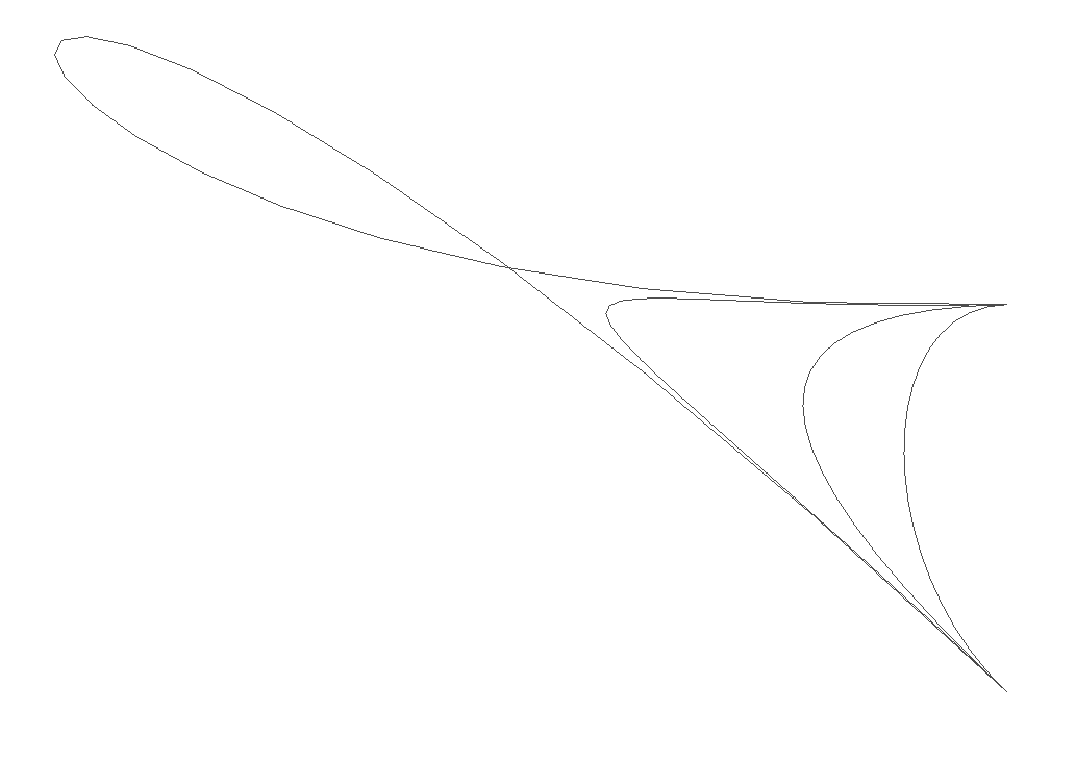
\includegraphics[width=\linewidth,height=0.87\linewidth]{chapter-05/figs/hermitecurves.pdf}%
	\end{minipage}%
	\begin{minipage}[c]{0.5\linewidth}
   	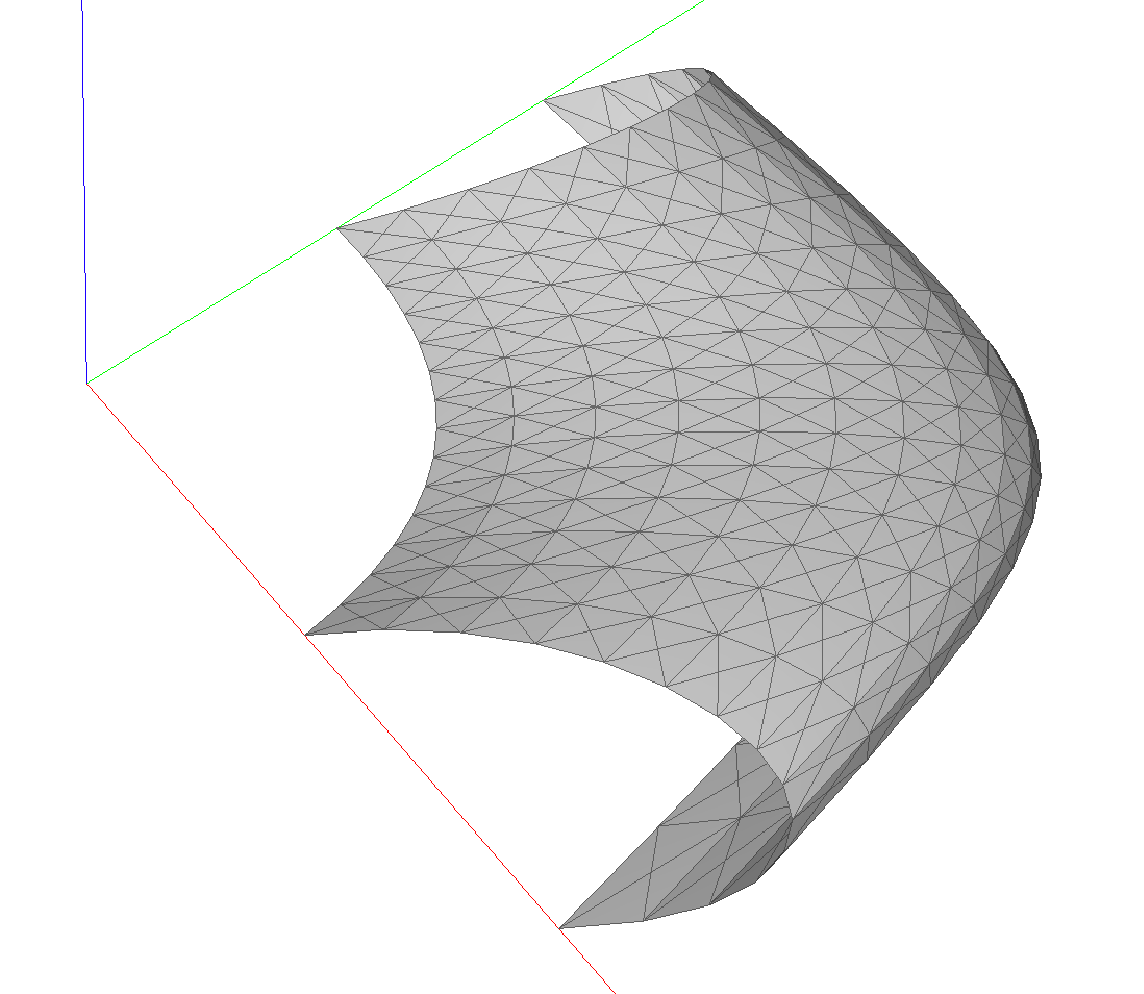
\includegraphics[width=\linewidth]{chapter-05/figs/trasfinitehermite.pdf}%
	\end{minipage}%

	\begin{minipage}[c]{0.5\linewidth}
   	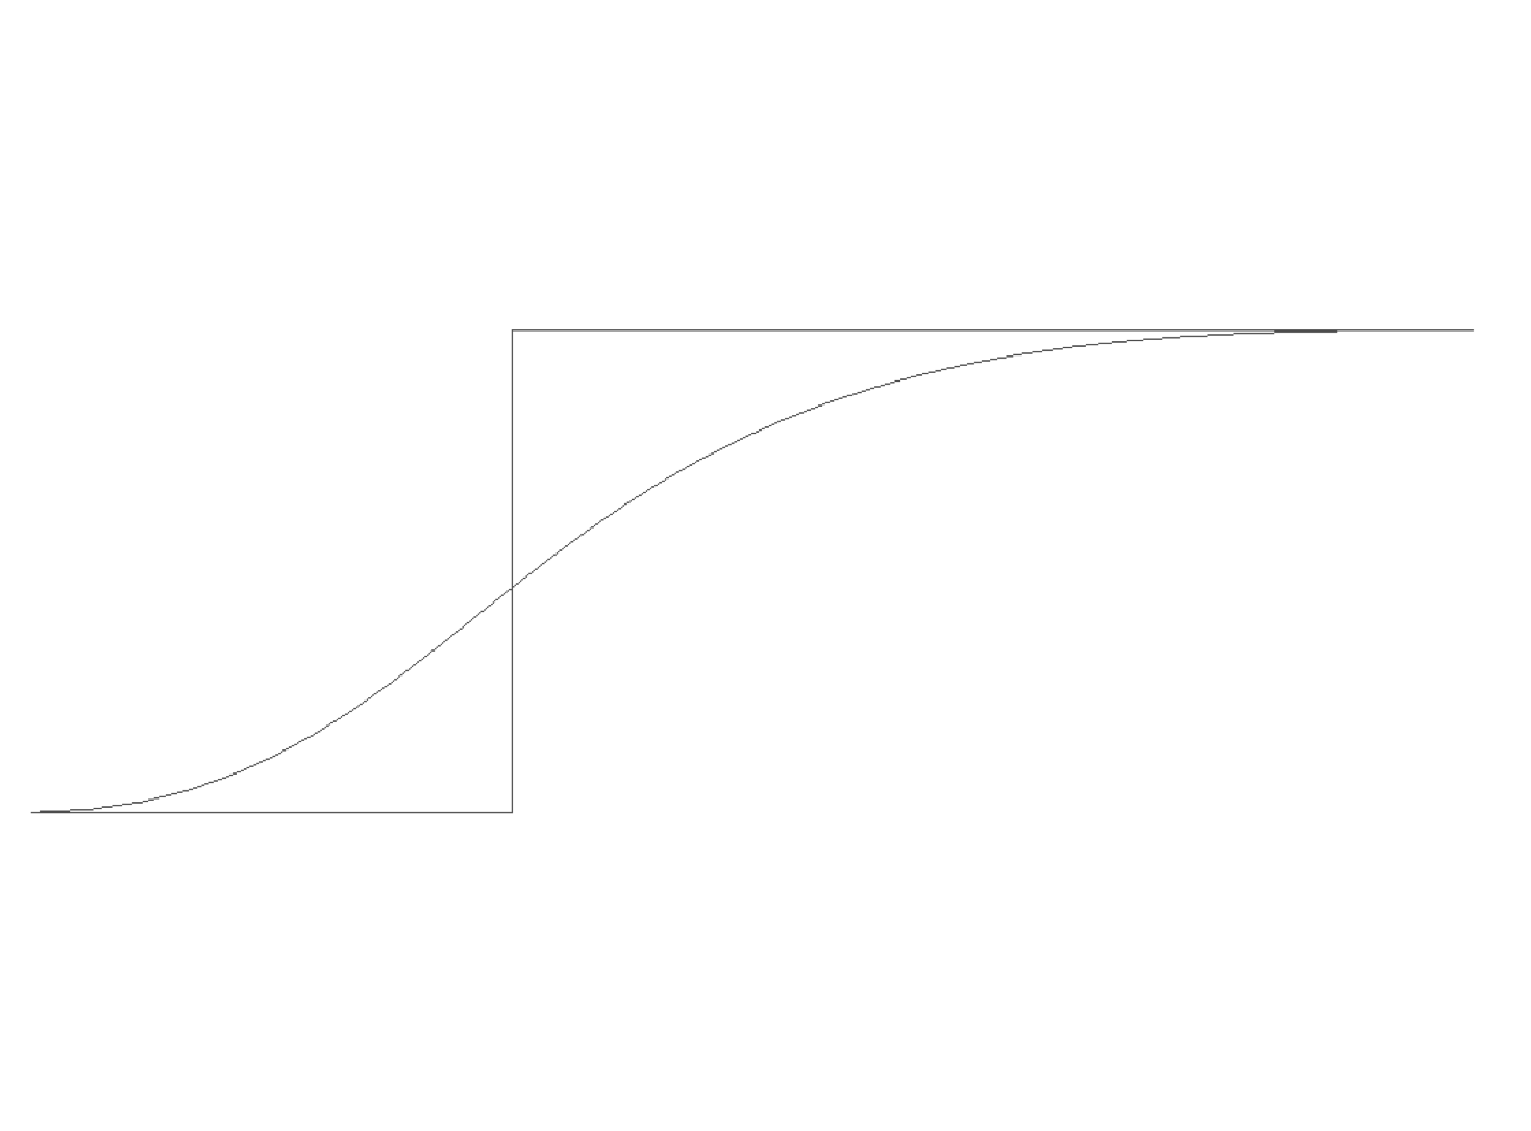
\includegraphics[width=\linewidth]{chapter-05/figs/bezier.pdf} 
	\end{minipage}%
	\begin{minipage}[c]{0.5\linewidth}
   	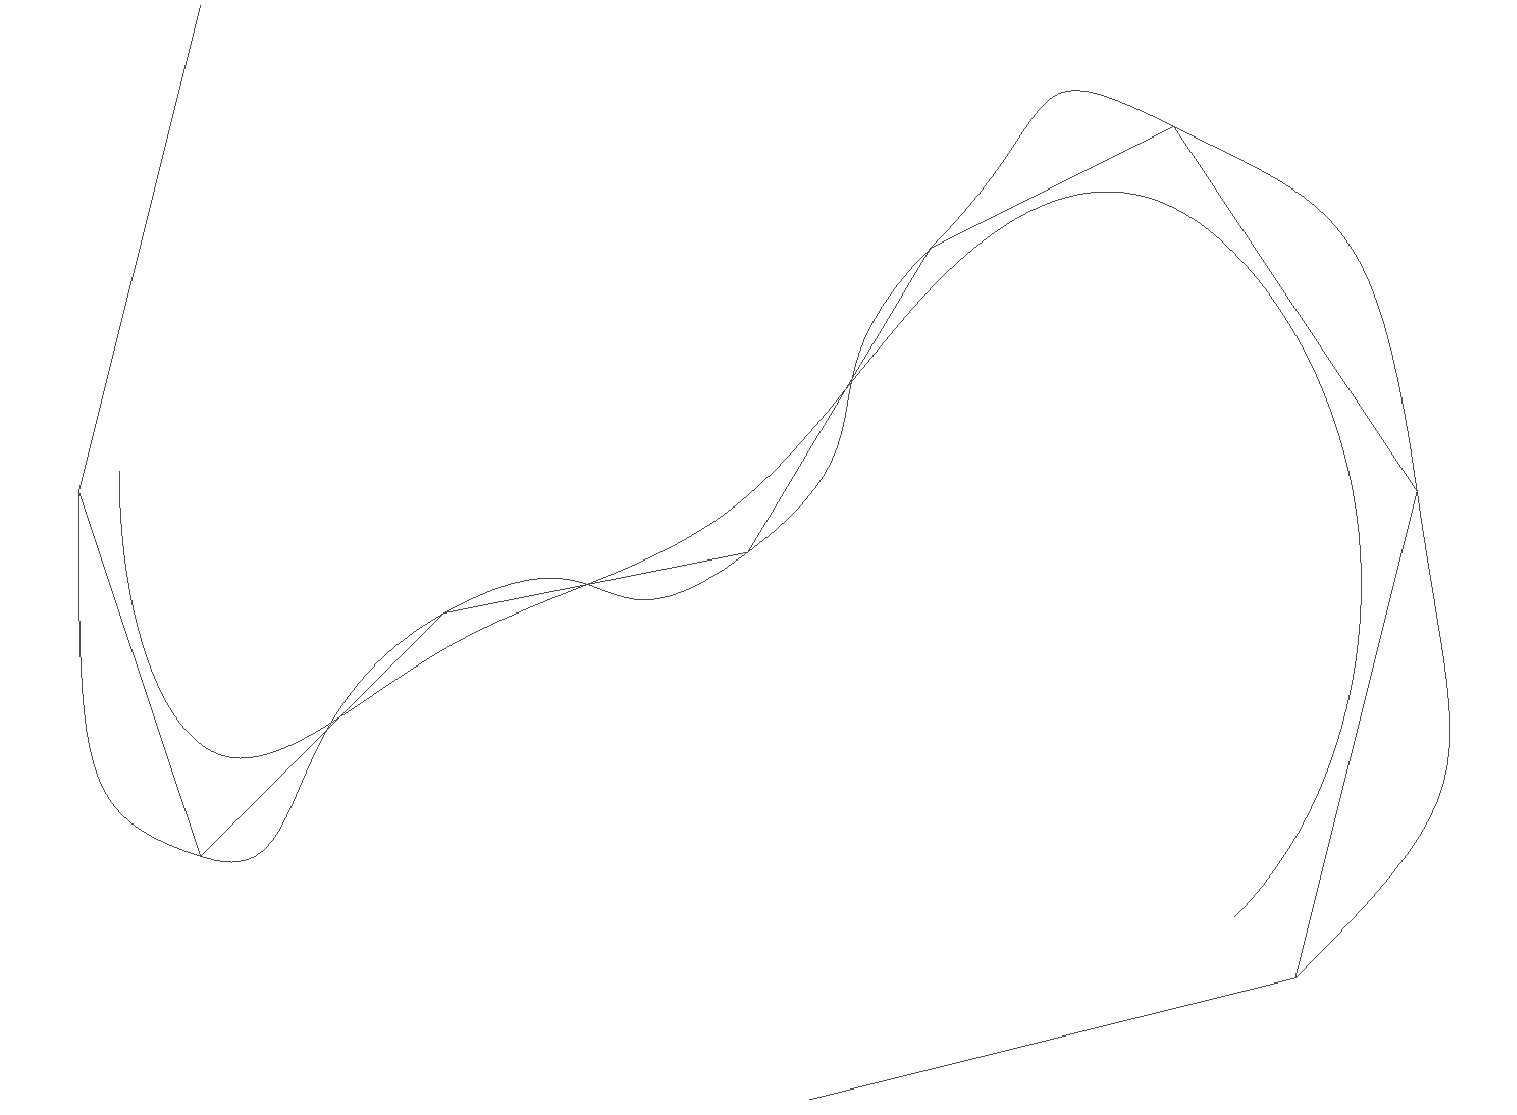
\includegraphics[width=\linewidth]{chapter-05/figs/nubspline.pdf} 
	\end{minipage}%

   \caption{Curve examples: (a) Hermite curves with same extreme point, and scaled extreme tangents (see Example \ref{ex:5:4:2}); (b) aaaaa aaaa aaaaaaa aaaaa aaaa aaaaaaa aaaaa aaaa aaaaaaa aaaaa aaaa aaaaaaa aaaaa aaaa aaaaaaa aaaaa aaaa aaaaaaa (see Example \ref{ex:5:4:3}); (c) aaaaa aaaa aaaaaaa aaaaa aaaa aaaaaaa aaaaa aaaa aaaaaaa aaaaa aaaa aaaaaaa aaaaa aaaa aaaaaaa aaaaa aaaa (see Example \ref{ex:5:4:4}); (d) aaaaa aaaa aaaaaaa aaaaa aaaa aaaaaaa aaaaa aaaa aaaaaaa aaaaa aaaa aaaaaaa aaaaa aaaa aaaaaaa aaaaa aaaa (see Example \ref{ex:5:4:4}). }
   \label{fig:5:7}
\end{figure}


\subsection{ Curve generation methods}\label{sect:5-4-1}

The primary |Plasm| generator of curves is the second order |MAP(curve::Function)(domain::Hpc)| combinator function. 

\begin{remark}[Semantics of {\sf MAP} operator]
The first argument function of the |MAP| combinator will extract the |1D| points from the polyhedral complex decomposition of the curve |domain|, second argument of the |MAP| operator. The mapped points remain embedded in |dom|, changing its shape, but not its topology, including connectness.
\end{remark}


\begin{condition}[(Hermite cubic curve] (See Figure~\ref{fig:5:7}a)
In the case of Hermite cubic curves four constraints impose the passage through assigned initial and final points (|P1|, |P2|), with assigned initial and final tangents (|T1|,|T2|). Four constraints, hence degree 3. The |Plasm| implementation is given below
\begin{lstlisting}[language=JuliaLocal, style=julia, mathescape=true]
function HERMITE(args)
	P1, P2, T1, T2 = args
	return CUBICHERMITE(S1)([P1, P2, T1, T2])
end
\end{lstlisting}
\end{condition}

\begin{condition}[Hermite cubic curve]\label{ex:5:4:2} (See Figure~\ref{fig:5:7}a)
We see here four |CUBICHERMITE| curves, with growing values of extreme tangents. At some point the curve self-intersect, which is bad for geometric design. Anyway, the low-degree Hermite curve are useful to use in spline, where to interpolate long sequences of points and tangents.
\begin{lstlisting}[language=JuliaLocal, style=julia, mathescape=true]
domain = INTERVALS(1.0)(20)
VIEW( STRUCT([		# aggregation of four curves
MAP(CUBICHERMITE(S1)([[1,0],[1,1],[ -1, 1],[ 1,0]]))(domain),
MAP(CUBICHERMITE(S1)([[1,0],[1,1],[ -2, 2],[ 2,0]]))(domain),
MAP(CUBICHERMITE(S1)([[1,0],[1,1],[ -4, 4],[ 4,0]]))(domain),
MAP(CUBICHERMITE(S1)([[1,0],[1,1],[-10,10],[10,0]]))(domain)]))
\end{lstlisting}
\end{condition}

\begin{condition}[(Transfinite Hermite surface] (See Figure~\ref{fig:5:7}b)
\label{\ref{ex:5:4:3}}
The transfinite Hermite implementation of Julia |Plasm| is used here.
Let us note that |c1| and |c2| are curves, since their expressions contain the |S1| selector; conversely, |sur3| is a surface, since contains |S2|. The two extreme curves are interpolated here. Of course, the |domain| is 2D, obtained as Cartesian product of two polyhedral complexes of dimension one.
\begin{lstlisting}[language=JuliaLocal, style=julia, mathescape=true]
c1 = CUBICHERMITE(S1)([[1  ,0,0],[0  ,1,0],[0,3,0],[-3,0,0]])
c2 = CUBICHERMITE(S1)([[0.5,0,0],[0,0.5,0],[0,1,0],[-1,0,0]])
cubic = CUBICHERMITE(S2)([c1,c2,[1,1,1],[-1,-1,-1]])		
# cubic : domain $\to \E^2$
domain = INTERVALS(1.0)(14) * INTERVALS(1.0)(14)
VIEW( MAP(cubic)(domain)), Dict("background_color"=>WHITE))
\end{lstlisting}
\end{condition}



\begin{definition}[Bézier curve]
Bézier curves of degree $n$ are entirely defined by an ordered sequence of $n+1$ control points. Such curves enjoy several useful properties, including (a) the interpolation of the first and last control point, and (b) the curve containment in the convex hull of |controlpoints|.  
\end{definition}
With two control points, we have a linear curve, three a quadratic curve, four a cubic curve, and so on. A cubic Bézier may have one flex (bend) point, a quartic two, a $n$-degree $n-2$ such points, so the shape is \emph{flexible}. For numerical reasons, it is better to maintain a low curve degree.

%///////////////////////////////////////////////////////////////////////////////
\begin{condition}[(Bézier quartic curve] (See Figure~\ref{fig:5:7}c)\
\label{\ref{ex:5:4:4}}
This script shows the first simple example of the important class of Bézier curves.  The curve |domain| is here a partition into |32| segments of the interval $[0,1]$. Thr degree of curve is 4 because of 5 control points.
\begin{lstlisting}[language=JuliaLocal, style=julia, mathescape=true]
controlpoints = [[0,0],[1,0],[1,1],[2,1],[2,2]]
curve  = BEZIER(S1)(controlpoints)
domain = INTERVALS(1.0)(32)

VIEW( STRUCT(MAP(curve)(domain), POLYLINE(controlpoints), FRAME2), Dict("background_color"=>WHITE) ) 
\end{lstlisting}
\end{condition}

\begin{definition}[Spline curve]
A \emph{spline} is a continuous curve constructed so as to pass through a given set of points and have a certain number of continuous derivatives. Splines may be either interpolating or approximating the control points. Each coordinate of control points generates a coordinate function of the curve.
\end{definition}

%///////////////////////////////////////////////////////////////////////////////
\begin{condition}[(Cubic spline curves] (See Figure~\ref{fig:5:7}d)\
\label{\ref{ex:5:4:5}}
Here we show two examples of 2D cubic splines, piecewise curve defined by joining several segments of low-degree curve. In case of cubic splines each consecutive quadruple of points defines a different curve segment. In Figure~\ref{} we see together the |polyline|  of control points, a cardinal (interpolating) and a uniform B-spline (approximating) curve.
\begin{lstlisting}[language=JuliaLocal, style=julia, mathescape=true]
domain = INTERVALS(1.0)(20)
points = [[-3.0, 6.0], [-4.0, 2.0], [-3.0,-1.0], [-1.0, 1.0], [1.5, 1.5], [3.0, 4.0], [5.0, 5.0], [7.0, 2.0], [6.0,-2.0], [2.0,-3.0]]
polyline = POLYLINE(points) 
cardinal_spline = SPLINE(CUBICCARDINAL(domain))(points);
uniform_Bspline = SPLINE(CUBICUBSPLINE(domain))(points);

VIEW( STRUCT( polyline, cardinal_spline, uniform_Bspline ) )
\end{lstlisting}
\end{condition}


%///////////////////////////////////////////////////////////////////////////////
\begin{condition}[(Exact ellipse curve] (See Figure~\ref{}a)\
Exact ellipse curve, whose quarter is generated as exact quadratic rational Bézier curvehown here s is. The example shows one of two ellipses degenerating to a rational circle. The are three control points because each quarter is a cubic Bezier curve.
\begin{lstlisting}[language=JuliaLocal, style=julia, mathescape=true]
function ELLIPSE(args::Vector{Float64})
	A, B = args
	function ELLIPSE0(N::Int)
		C = 0.5*sqrt(2)
		mapping = RATIONALBEZIER([[A, 0.0, 1.0], [A*C, B*C, C], 		[0.0, B, 1.0]])
		quarter = MAP(mapping)((INTERVALS(1.0)(N)))
		half = STRUCT([quarter, S(2)(-1.0)(quarter)])
		return STRUCT([half, S(1)(-1.0)(half)])
	end
	return ELLIPSE0
end

VIEW( STRUCT( ELLIPSE([1.0,2.0])(15), ELLIPSE([2.0,2.0])(15) ) )
\end{lstlisting}
\end{condition}

%///////////////////////////////////////////////////////////////////////////////
\begin{condition}[(Non Uniform cubic B-spline] (See Figure~\ref{}a)\
This class of splines has consecutive curve segments defined between pairs of consecutive parameter values, called \emph{knots}. To interpolate the extreme control points, the extreme knots must have \emph{multiplicity} equal to $degree + 1$. 

In this example, for the number of control points we have $n = m - (degree + 1) = 14 - 4 = 10$, where $m = n+degree+1$ is the number of knots. The number of cubic curve segments is $n - degree = 7$.  The knots are not necessarily integer. The knots (in parameter space) may be subject of affine maps (translation and scaling.

\begin{lstlisting}[language=JuliaLocal, style=julia, mathescape=true]
degree = 3
ControlPoints = [[0.,0],[-1,2],[1,4],[2,3],[1,1],[1,2],[2.5,1],[2.5,3],[4,4],[5,0]]  
# 10 control points
knots=[0,0,0,0, 1,2,3,4,5,6, 7,7,7,7] # 14 knots
VIEW(DISPLAYNUBSPLINE(degree, knots, ControlPoints))
\end{lstlisting}
\end{condition

\begin{remark}
As a rule of thumb, start fixing the control points and, hence, the approximate spline shape by viewing their |POLYLINE|. Choose the degree and, consequently, the number of curve segments and knots ($m=n+degree+1$). Finally, write the knot sequence starting from zero and repeat $n+1$ times, then append a knot at a time until it reaches the number of segments, and repeat the last knot.
Other examples of |NUBSPLINE| (non rational NURBS) with 10 control points are given below:

n=10; degree=2; segments=8; m=13 ; knots=0,0,0, 1,2,3,4,5,6,7, 8,8,8 

n=10; degree=4; segments=6; m=15 ; knots=0,0,0,0,0 1,2,3,4,5, 6,6,6,6,6 }\\
\end{remark}


%///////////////////////////////////////////////////////////////////////////////
\begin{condition}[(Quadratic NURBS circle] (See Figure~\ref{}a)\
There are several ways to construct an exact 1D circle with NURBS curves of degrees two, three, and \four~\cite{Eberly/ww.geometrictools.com/}. In the case implemented in this example (see also Figure~\ref{}) we have
$n=9 (2 coincidenti), degree=2, m=12$ satisfying our parameter relation formulas:
\begin{lstlisting}[language=JuliaLocal, style=julia, mathescape=true]
knots = [0,0,0,1,1,2,2,3,3,4,4,4]
_p=sqrt(2)/2.0
controlpoints = [[-1,0,1], [-_p,_p,_p], [0,1,1], [_p,_p,_p],[1,0,1], [_p,-_p,_p], [0,-1,1], [-_p,-_p,_p], [-1,0,1]]
VIEW(MAP: DISPLAYNURBSPLINE([2, knots, controlpoints])(domain), Dict("background_color"=>WHITE))
\end{lstlisting}
\end{condition}


%$$$$$$$$$$$$$$$$$$$$$$$$$$$$$$$$$$$$$$$$$$$$$$$$$$$$$$$$$$$$$$$$$$$$$$$$$$$$$$$
\subsection{ Surface generation methods}\label{sect:5-4-2}
%$$$$$$$$$$$$$$$$$$$$$$$$$$$$$$$$$$$$$$$$$$$$$$$$$$$$$$$$$$$$$$$$$$$$$$$$$$$$$$$

Parametric curves can be combined to give parametric surfaces or
solids or higher dimensional manifolds.  In this section we introduce \emph{generative methods} for parametric surfaces as
vector functions of two real parameters, but also presents extensions
to some three-variate solids.  Useful classes of surfaces are discussed, i.e.~the \emph{profile
product} surfaces, including rotational surfaces; the \emph{ruled}
surfaces, including generalized cylinders and cones; the surfaces
generated by \emph{tensor product} of curves or splines. 
The simple combinatorial semantics of the |Plasm| language
may give the reader useful insights into tensor operations and
transfinite combinations.


To generate a 2D surface, i.e. a 2-dimensional manifold embedded in $\E^3$, we have to produce a vector-valued function with 3 coordinate functions $S(u,v) = [x(u,v), y(u,v), z(u,v)]$.


%///////////////////////////////////////////////////////////////////////////////
\begin{condition}[(Parametric sphere] (See Figure~\ref{}a)\
A unit sphere centered in the origin is given here. the default |domain| is a cell  decomposition of the $[0,\pi] \times [0,2\pi]$ rectangle into $16\times 32$ quads.
The |SPHERE| generating function in 3D is quickly generated as |Hpc| with some empty triangles at poles and double vertices and edges at the $v$ edges of $u,v$ discretized domain. 
\begin{lstlisting}[language=JuliaLocal, style=julia, mathescape=true]
function SPHERE(radius=1.0::Number)
   function SPHERE0(subds=[16,32]::Vector{Int})
      N, M = subds
      dom = INTERVALS(π)(N) * INTERVALS(2π)(M)
      domain = T(1,2)(-π/2,-π)(dom)
      fx = p -> radius * (-cos(p[1])) * sin(p[2])
      fy = p -> radius * cos(p[1]) * cos(p[2])
      fz = p -> radius * sin(p[1])
      return MAP([fx, fy, fz])(domain)
   end
   return SPHERE0
end
\end{lstlisting}
A |SPHERE| surface with unit radius and piecewise-linearly approximated by  $16\times 32$ quads (default) is given here:
\begin{lstlisting}[language=JuliaLocal, style=julia, mathescape=true]
VIEW( SPHERE(1.0)([16,32]), Dict(“background_color”=>WHITE) )
\end{lstlisting}
In order to curate the |Hpc| surface from empty triangles and double vertices and edges,
the sphere representation must be ported to |Lar| data structure.
Maximum correct refinement is |LAR(SPHERE(2)([73,40]))|.
\end{condition}

%///////////////////////////////////////////////////////////////////////////////
\begin{condition}[(Parametric torus] (See Figure~\ref{}a)\
The parametric equation of torus surface in 3D can be computed by rotating about the $z$ axis a parametric circle in the plane x=0. The reader may construct it by exercise. The three coordinate functions are called |fx, fy, fz|, The |domain| is $[0,2\pi]\times[2\pi]$. The surface depends on a minor and a major radii (|r1|, |r2|).

The |TORUS|, function of second order, is given below.
Instead than using a |Plasm| vector function |CONS([x,y,z])∘S1| a different technique is used here, by mapping a vector $of$ bivariate functions of |p = (u,v)| on the 2D |domain|.
\begin{lstlisting}[language=JuliaLocal, style=julia, mathescape=true]
function TORUS(radii=[1.0,2]::Vector)
	r1, r2 = radii
	function TORUS0(subds=[16,32]::Vector{Int})
		N, M = subds
		a = 0.5 * (r2-r1)
		c = 0.5 * (r1+r2)
		domain = INTERVALS(2*pi)(N) * INTERVALS(2*pi)(M)
		fx = p -> (c + a*cos(p[2])) * cos(p[1])
		fy = p -> (c + a*cos(p[2])) * sin(p[1])
		fz = p -> a * sin(p[2])
		return MAP([fx, fy, fz])(domain)
	end
	return TORUS0
end
\end{lstlisting}
An application example of the |TORUS| function to actual parameters follows. 
|[1.0,2.0]| are the smaller and bigger radii.
\begin{lstlisting}[language=JuliaLocal, style=julia, mathescape=true]
VIEW( TORUS([1.0,2.0])([20,80]),Dict("background_color"=>WHITE ) 
\end{lstlisting}
\end{condition}

%///////////////////////////////////////////////////////////////////////////////
\begin{condition}[(Cubic Bézier surface generated by Bézier curves] (See Figure~\ref{}a)\ 

A transfinite generation is given here, where the four parameters of a cubic Bézier manifold are given by |C0,C1,C2,C3| Bézier’s curves of various degrees.
\begin{lstlisting}[language=JuliaLocal, style=julia, mathescape=true]
C0 = BEZIER(S1)([[0,0,0],[10,0,0]])
C1 = BEZIER(S1)([[0,2,0],[8,3,0],[9,2,0]])
C2 = BEZIER(S1)([[0,4,1],[7,5,-1],[8,5,1],[12,4,0]])
C3 = BEZIER(S1)([[0,6,0],[9,6,3],[10,6,-1]])
domain = INTERVALS(1.0)(10) * INTERVALS(1.0)(10)
VIEW(MAP(BEZIER(S2)([C0,C1,C2,C3]))(domain))
\end{lstlisting}
\end{condition}


%///////////////////////////////////////////////////////////////////////////////
\begin{condition}[(Coons’ patch] (See Figure~\ref{}a)\
The Coons patch provides a method to construct a surface supported on a given contour, when the latter is composed of 4 arcs of curves.
\begin{lstlisting}[language=JuliaLocal, style=julia, mathescape=true]
Su0 = BEZIER(S1)([[0,0,0],[10,0,0]])
Su1 = BEZIER(S1)([[0,10,0],[2.5,10,3],[5,10,-3],[7.5,10,3],[10,10,0]])
Sv0 = BEZIER(S2)([[0,0,0],[0,0,3],[0,10,3],[0,10,0]])
Sv1 = BEZIER(S2)([[10,0,0],[10,5,3],[10,10,0]])
domain = INTERVALS(1.0)(10) * INTERVALS(1.0)(10)
VIEW(MAP(COONSPATCH([Su0,Su1,Sv0,Sv1]))(domain))
\end{lstlisting}
\end{condition}

%///////////////////////////////////////////////////////////////////////////////
\begin{condition}[(Ruled surface] (See Figure~\ref{}a)\
The |RULEDSURFACE| function is used to build a ruled 2-manifold between two given curves. Of course, the domain must be 2D ,and embedded in a Euclidean space of at least dimension $d=2$.
\begin{lstlisting}[language=JuliaLocal, style=julia, mathescape=true]
alpha = point -> [point[1], point[1], 0 ]
beta = point -> [ -1,  +1, point[1] ]
domain = T([1,2])([-1,-1])(INTERVALS(2.0)(10) * INTERVALS(2.0)(10))
VIEW( MAP(RULEDSURFACE([alpha,beta]))(domain) )
\end{lstlisting}
The two parametric functions |alpha| and |beta| define a patch  of hyperbolic paraboloid surface, with two parametric maps $\E^2\to\E^3$ such that $(u,v)\mapsto[u,u,0]$ and $(u,v)\mapsto[-1,1,u]$ over the |domain| patch $$|T|(1,2)(-1.-1)([0,2]\times[0,2])=([-1,1]\times[-1,1])\subset\E^2$$.
A hyperbolic paraboloid is a saddle surface (see Figure~\ref{}), as its Gauss curvature is negative at every point. Therefore, although it is a ruled surface, it is not developable. 
\end{condition}

%///////////////////////////////////////////////////////////////////////////////
\begin{condition}[(Profile product patch] (See Figure~\ref{}a)\ A similar development pattern is used here, using a profile curve and a section curve. A rotational curve is a |profile| product with a circle |section|. A surface $\p{S}$ is called the {\it profile
product} of two plane curves $\p{\alpha}$ and $\p{\beta}$, embedded
into two coordinate subspaces and respectively called {\it profile}
and {\it cross-section} curve:
\[ 
\p{\alpha}(u) = \vet{\alpha_1(u) & 0 & \alpha_3(u)}^{T}, \quad
\p{\beta}(v) = \vet{\beta_1(v) & \beta_2(v) & 0}^{T}
\]
when it is of the form
\[
\p{S}(u,v) = 
\vet{\alpha_1(u)\ \beta_1(v), \  \alpha_1(u)\ \beta_2(v), \  
\alpha_3(u)}^{T}
\]
\begin{lstlisting}[language=JuliaLocal, style=julia, mathescape=true]
profile = BEZIER(S1)([[0.1,0,0],[2,0,0],[0,0,4],[1,0,5]])
section = BEZIER(S2)([[0,0,0],[3,-0.5,0],[3,3.5,0],[0,3,0]])
domain = INTERVALS(1.0)(20) * INTERVALS(1.0)(20)
VIEW( STRUCT( MAP(profile)(domain), MAP(section)(domain) ), Dict(background_color=>WHITE)”)
VIEW( MAP(PROFILEPRODSURFACE([profile, section])(domain) ))
\end{lstlisting}
\end{condition}

%///////////////////////////////////////////////////////////////////////////////
\begin{condition}[(Rotational surface and solid] (See Figure~\ref{}a)\
The primitive function |ROTATIONALSURFACE| is a profile product where the |section| function is already known. The control points of the |profile| curve are set to start with horizontal tangent vector at $u=0$. Of course, the |profile| curve rules entirely the surface shape. In figures \ref{} and \ref{} we show both the rotational surface and the thin solid derived from it.
\begin{lstlisting}[language=JuliaLocal, style=julia, mathescape=true]
profile = BEZIER(S1)([[0,0,0],[3,0,0],[4,0,1],[4,0,4]]) 
domain = INTERVALS(1.0)(10) * INTERVALS(2*PI)(30)
suface = ROTATIONALSURFACE(profile)
VIEW( MAP(suface)(domain) )
VIEW( MAP(THINSOLID(suface))(domain*INTERVALS(0.25)(1))) 
\end{lstlisting}
\end{condition}

%///////////////////////////////////////////////////////////////////////////////
\begin{condition}[(Cylindrical surface and solid] (See Figure~\ref{}a)\
A cilindrical surface is given here implemented by the |CYLINDRICALSURFACE| primitive by tensor product of a Bézier curve |alpha| in $z=0$ and a vertical vector |[0,0,1]|. 
\begin{lstlisting}[language=JuliaLocal, style=julia, mathescape=true]
alpha = BEZIER(S1)([[1,1,0],[-1,1,0],[1,-1,0],[-1,-1,0]])
Udomain = INTERVALS(1.0)(20)
Vdomain = INTERVALS(1.0)(6)
domain = Udomain * Vdomain
fn = CYLINDRICALSURFACE([alpha,[0,0,1]])
VIEW(MAP(fn)(domain))
VIEW(MAP(THINSOLID(fn))(domain*Vdomain))
\end{lstlisting}
\end{condition}

%///////////////////////////////////////////////////////////////////////////////
\begin{condition}[(Conical surface] (See Figure~\ref{}a)\
A conical surface is a ruled surface whose straight lines join a base curve, the |beta| Bézier in this example and a fixed point, in this case |[0,0,1]| out of the curve.
\begin{lstlisting}[language=JuliaLocal, style=julia, mathescape=true]
domain = Power(INTERVALS(1.0)(20),INTERVALS(1.0)(6))
beta = BEZIER(S1)([ [1,1,0],[-1,1,0],[1,-1,0],[-1,-1,0] ])
VIEW(MAP(CONICALSURFACE([[0,0,1],beta]))(domain), Dict("background_color"=>WHITE))
\end{lstlisting}
\end{condition}

\begin{definition}[Tensor product surface]
The parametric surfaces called \emph{tensor product surfaces} are a
bivariate generalization of parametric curves, e.g., 
polynomial surfaces are a linear combination of either points or
vectors with a suitable basis of \emph{bivariate} polynomial
functions.  
\end{definition}
Such a bivariate basis is obtained by \emph{tensor product}
of two univariate bases.  Let us remember that the basis of tensor product of two function bases (say, univariate Hermite o Bézier) can be obtained as $m\times n$ matrix product of first basis as $m\times 1$ column-vector times the second basis as $1\times n$ row-vector. 

The result of the linear combination of so generated 
bivariate basis with a $m\times n$ set of geometric handles is a point-valued
function of two real parameters, whose image set is the surface
considered as a point locus. 
 
The following examples show more than one generation method in action, encouraging the reader to reason about and distinguish between bivariate parametric surface functions, coordinate functions, transfinite combinations, and polynomial tensor product functions, which are directly mapped on $ m \times n$ matrices of control points. In some cases, the interested reader will directly look at the open-source implementation of the primitive functions.

%///////////////////////////////////////////////////////////////////////////////
\begin{condition}[(Transfinite Hermite surface] (See Figure~\ref{}a)\
In this case we present a cubic transfinite Hermite interpolating two |CUBICHERMITE| curves, and with two constant ($u$) fields (initial and final), of partial derivatives in the $v$ directions (see Figure \ref{}).
 \begin{lstlisting}[language=JuliaLocal, style=julia, mathescape=true]
c1 = CUBICHERMITE(S1)([[1,0,0],[0,1,0],[0,3,0],[-3,0,0]])
c2 = CUBICHERMITE(S1)([[0.5,0,0],[0,0.5,0],[0,1,0],[-1,0,0]])
sur3 = CUBICHERMITE(S2)([c1,c2,[1,1,1],[-1,-1,-1]])
domain = INTERVALS(1.0)(14) * INTERVALS(1.0)(14)
VIEW( MAP(sur3)(domain), Dict("background_color"=>WHITE) )
\end{lstlisting}
\end{condition}


%///////////////////////////////////////////////////////////////////////////////
\begin{condition}[(Bilinear surface] (See Figure~\ref{}a)\
Tensor product surface function generated by the |Plasm| operator |TENSORPRODUCT| with arguments two array of 3D |controlpoints|, each containing two points, the first and the last of a linear curve in one parametric direction. the same for the transposed tensor in the other parametric coordinate direction. It is the ruled surface generated by four given points, that is interpolated at the four extreme points of |domain| $[0,1]\times[0,1]$. 

\begin{lstlisting}[language=JuliaLocal, style=julia, mathescape=true]
controlpoints = [
   [[0.0,0.0,0.0],[2.0,-4.0,2.0]],
   [[0.0,3.0,1.0],[4.0,0.0,0.0]]] .* 0.25
domain = INTERVALS(1.0)(10) * INTERVALS(1.0)(10)
mapping = BILINEARSURFACE(controlpoints)
VIEW( MAP(mapping)(domain), Dict("background_color"=>WHITE) )
\end{lstlisting}
The |Plasm| implementation of the |BILINEARSURFACE| operator follows. The
|BERNSTEINBASIS| of first degree is just the convex combinator of two control points: $[1-u, u]$.
\begin{lstlisting}[language=JuliaLocal, style=julia, mathescape=true]
function BILINEARSURFACE(controlpoints)
	return TENSORPRODSURFACE([BERNSTEINBASIS(S1)(1), BERNSTEINBASIS(S1)(1)])(controlpoints)
end
\end{lstlisting}
\end{condition}

%///////////////////////////////////////////////////////////////////////////////
\begin{condition}[(Biquadratic surface] (See Figure~\ref{}a)\
The operator, in this case\\ |BIQUADRATICSURFACE|, is generated by |TENSORPRODSURFACE| of two instances of  quadratic Bézier , given as 
$basis = [ (1-u)^{2},\ 2(1-u)u,\ u^{2} ]\ (0\leq u\leq 1).$

\begin{lstlisting}[language=JuliaLocal, style=julia, mathescape=true]
controlpoints = [[[0,0,0],[2,0,1],[3,1,1]],[[1,3,-1],[3,2,0],[4,2,0]],[[0,9,0],[2,5,1],[3,3,2]]]
domain = INTERVALS(1.0)(10) * INTERVALS(1.0)(10)
mapping = BIQUADRATICSURFACE(controlpoints)
VIEW(MAP(mapping)(domain), Dict("background_color"=>WHITE))
\end{lstlisting}
\end{condition}



%///////////////////////////////////////////////////////////////////////////////
\begin{condition}[(Bicubic Hermite surface] (See Figure~\ref{}a)\
Theis surface is an extension of Hermite curve. It is defined by 16 parameters (4 end points, 8 tangent vectors at end points, 4 twist vectors). You have (a) position vectors: the four corner points; (b) tangent vectors: the tangent vectors in u, w directions at the four position vectors of the surface; (c) twist vectors: the twist vectors at all the four position vectors of the surface. The elements of |controlpoints| tensor can be put in correspondence with the function of the basis tensor:

\[
\T{\cal G}_{hh} = \mat{
\T{S}(0,0) & \T{S}(0,1) && \T{S}^u(0,0) & \T{S}^u(0,1) \\
\T{S}(1,0) & \T{S}(1,1) && \T{S}^u(1,0) & \T{S}^u(1,1) \\ \\
\T{S}^v(0,0) & \T{S}^v(0,1) && \T{S}^{uv}(0,0) & \T{S}^{uv}(0,1) \\
\T{S}^v(1,0) & \T{S}^v(1,1) && \T{S}^{uv}(1,0) & \T{S}^{uv}(1,1) 
}
\]
It is easy to see that the |controlpoints| geometric tensor $\T{\cal G}_{hh}$ can be decomposed into four submatrices corresponding to the surface $\T{S}$, its first partial
derivatives $\T{S}^u$, $\T{S}^v$ and its mixed second partial derivative $\T{S}^{uv}$, called twist vectors, respectively evaluated in the four corners of [0,1]^{2}$ domain:

\begin{lstlisting}[language=JuliaLocal, style=julia, mathescape=true]
controlpoints = [
   [[0,0,0 ],[2,0,1], [3,1,1],[4,1,1]],
   [[1,3,-1],[3,2,0], [4,2,0],[4,2,0]],
   
   [[0,4,0 ],[2,4,1], [3,3,2],[5,3,2]],
   [[0,6,0 ],[2,5,1], [3,4,1],[4,4,0]]
]
domain = INTERVALS(1.0)(10) * INTERVALS(1.0)(10)
mapping = HERMITESURFACE(controlpoints)
VIEW( MAP(mapping)(domain), Dict("background_color"=>WHITE) )
\end{lstlisting}
\end{condition}

%///////////////////////////////////////////////////////////////////////////////
\begin{condition}[(Bicubic Beziér surface] (See Figure~\ref{}a)\
Conversely, the generating |controlpoints| of a cubic Bézier surface in 3D are a $4\times 4$ matrix of 3D point coordinates. This kind of suface interpolates the four extreme points, and the two cubic curves generated by the first and last row, as well the two cubic curves generated by the first and last column of the tensor of points.  
\begin{lstlisting}[language=JuliaLocal, style=julia, mathescape=true]
controlpoints = [
   [[ 0,0,0],[0 ,3  ,4],[0, 6, 3],[0,10,0]],
   [[ 3,0,2],[2 ,2.5,5],[3, 6, 5],[4,8,2]],
   [[ 6,0,2],[8 ,3 , 5],[7,6,4.5],[6,10,2.5]],
   [[10,0,0],[11,3  ,4],[11,6, 3],[10,9,0]]
]
domain = INTERVALS(1.0)(10) * INTERVALS(1.0)(10)
mapping = BEZIERSURFACE(controlpoints)
VIEW(MAP(mapping)(domain), Dict("background_color"=>WHITE))
\end{lstlisting}
\end{condition}

%///////////////////////////////////////////////////////////////////////////////
\begin{condition}[(From polyline 2D to polygon] (See Figure~\ref{}a)\
A polyline is a list of points, where line segments are drawn between consecutive points.  a polygon is the set on points of a 2D domain, whose boundary gives a closed polyline. A polyline is said closed when has no boundary points.
\begin{lstlisting}[language=JuliaLocal, style=julia, mathescape=true]
VIEW(SOLIDIFY(STRUCT(AA(POLYLINE)([
   [[0,0],[4,2],[2.5,3],[4,5],[2,5],[0,3],[-3,3],[0,0]],
   [[0,3],[0,1],[2,2],[2,4],[0,3]],
   [[2,2],[1,3],[1,2],[2,2]]]))), Dict("background_color"=>WHITE))
\end{lstlisting}
\end{condition}





%$$$$$$$$$$$$$$$$$$$$$$$$$$$$$$$$$$$$$$$$$$$$$$$$$$$$$$$$$$$$$$$$$$$$$$$$$$$$$$$
\subsection{ Solid generation examples}\label{sect:5-4-3}
%$$$$$$$$$$$$$$$$$$$$$$$$$$$$$$$$$$$$$$$$$$$$$$$$$$$$$$$$$$$$$$$$$$$$$$$$$$$$$$$

Here, we discuss several generations of 3D solids. In particular, we use the |TENSORPRODUCT| primitive, performing either the polynomial combination of two or more parametric curves or a parametric surface and a curve. Another method is called |SOLIDIFY| and consists of applying the same operation seen for the generation of solid polygons from closed and hollow polylines.
Another method, Minkowski projection, will be used with 4D solids to generate a 3D view through a central projection within one of their faces.

%///////////////////////////////////////////////////////////////////////////////
\begin{condition}[(CUBE primitive] (See Figure~\ref{}a)\
This primitive generator of the 3D cube has only one argument, the size of edges. 
\begin{lstlisting}[language=JuliaLocal, style=julia, mathescape=true]
cube = CUBE(3)
VIEW( cube, Dict("background_color"=>WHITE) )
\end{lstlisting}
\end{condition}


%///////////////////////////////////////////////////////////////////////////////
\begin{condition}[($d$-Permutahedron] (See Figure~\ref{}a)\ 
The permutahedron of order $d$ is a ($d−1$)-dimensional polytope embedded in $d$D space. It is the boundary of a $d$-solid generated by permutation of first $d$-integers. The examples of 2- and 3-permutahedra follow. The generating operator |PERMUTAHEDRON| is multidimensional, with $d\geq 2$.
\begin{lstlisting}[language=JuliaLocal, style=julia, mathescape=true]
VIEW( PERMUTAHEDRON(2), Dict("background_color"=>WHITE) )
VIEW( PERMUTAHEDRON(3), Dict("background_color"=>WHITE) )
\end{lstlisting}
\end{condition}


%///////////////////////////////////////////////////////////////////////////////
%\begin{condition}[(Schegel projection in 3D] (See Figure~\ref{}a)\
%The \emph{Schlegel diagram} of a polytope
%$P\subset\E^{d}$, with $\dim P = d$, is defined as the polytopal
%complex ${\cal S}(P, F, \p{y})$, of dimension $d-1$, which is obtained
%by projecting $P$ onto a facet $F\in{\cal F}(P)$ from an
%external point~$\p{y}$.
%In some sense, the Schlegel diagram ${\cal S}(P)$ encodes the
%combinatorial structure of a $d$-polytope $P$ into a $(d-1)$-complex
%${\cal S}(P)$.
%Such perspective transformation can be directly applied in \pl\ to a
%polyhedral domain by using the primitive operator \texttt{MAP}, as
%shown in Script~\ref{script:4:Schlegel}, where two different operators
%\texttt{schlegel2D} and \texttt{schlegel3D} are given, to generate the
%diagrams of 3D and 4D polytopes, respectively.
%
%
%\begin{lstlisting}[language=JuliaLocal, style=julia, mathescape=true]
%	VIEW(SCHLEGEL3D(0.2)((T([1,2,3,4])([-1.0/3.0,-1.0/3.0,-1,+1])(SIMPLEX(4)))), Dict("background_color"=>WHITE))
%	VIEW(SCHLEGEL3D(0.2)((SKELETON(1)∘T(1,2,3,4)(-1,-1,-1,1))(CUBOID([2,2,2,2])))), Dict("background_color"=>WHITE))
%	VIEW(SCHLEGEL3D(0.2)((T([1,2,3,4])([-1.0/3.0,-1.0/3.0,-1,+1])(Power(SIMPLEX(2),SIMPLEX(2))))), Dict("background_color"=>WHITE))
%\end{lstlisting}
%\end{condition}

%///////////////////////////////////////////////////////////////////////////////
\begin{condition}[(Quadratic Bézier 3-manifold] (See Figure~\ref{}a)\ In this case the fundamental function is |BEZIERMANIFOLD| that accepts the list of degrees in parametric coordinates $u,v,w$ and three second order tensors (in this case all $3\times 3\times 3$) that if assembled provide a 3-tensor of points. The result is a decomposed solid into a 3D grid, deformed according to the 3-tensor ox control points. 
\begin{lstlisting}[language=JuliaLocal, style=julia, mathescape=true]
grid1D = INTERVALS(1.0)(10)
domain3D = grid1D * grid1D *grid1D
degrees = [2,2,2]
Xtensor = [[[0,1,2],[-1,0,1],[0,1,2]],[[0,1,2],[-1,0,1],[0,1,2]], [[0,1,2],[-1,0,1],[0,1,2]]]
Ytensor = [[[0,0,0.8],[1,1,1],[2,3,2]], [[0,0,0.8],[1,1,1],[2,3,2]], [[0,0,0.8],[1,1,1],[2,3,2]]]
Ztensor = [[[0,0,0],[0,0,0],[0,0,0]],[[1,1,1], [1,1,1],[1,1,1]], [[2,2,1],[2,2,1],[2,2,1]]] 
mapping = BEZIERMANIFOLD(degrees)([Xtensor,Ytensor,Ztensor])
VIEW( MAP(mapping)(domain3D), Dict("background_color"=>WHITE) )
\end{lstlisting}
\end{condition}


%///////////////////////////////////////////////////////////////////////////////
\begin{condition}[(Minkowski sum of wireframe end cuboid] (See Figure~\ref{}a)
The example shows the offset of a 1D graph-like cell-complex. The solid kernel traveling along the edges of the wire frame model is a parallolopiped with sides $[0.1,0.2,0.1]$.
The generative algorithm works by using higher dimension (up to six) that the normal workspace $\E^3$.

\begin{lstlisting}[language=JuliaLocal, style=julia, mathescape=true]
verts = [[0,0,0],[3,0,0],[3,2,0],[0,2,0],[0,0,1.5], [3,0,1.5],[3,2,1.5],[0,2,1.5],[0,1,2.2],[3,1,2.2]]
cells = [[1,2],[2,3],[3,4],[4,1],[5,6],[6,7],[7,8],[8,5], [1,5],[2,6],[3,7],[4,8],[5,9],[8,9],[6,10],[7,10], [9,10]]
pols = [[1]]
House = MKPOL(verts,cells,pols)

VIEW( STRUCT( OFFSET([0.1,0.2,0.25])(House), T(2)(1.2*SIZE(2)(House))(House)), Dict("background_color"=>WHITE) )
\end{lstlisting}
\end{condition}


%///////////////////////////////////////////////////////////////////////////////
\begin{condition}[(aaaaaaa] (See Figure~\ref{}a)\
\begin{lstlisting}[language=JuliaLocal, style=julia, mathescape=true]
function TestThinSolid()
	Su0 = COMP([BEZIERCURVE([[0,0,0],[10,0,0]]),CONS([S1])])
	Su1 = COMP([BEZIERCURVE([[0,10,0],[2.5,10,3],[5,10,-3],[7.5,10,3],[10,10,0]]),CONS([S1]) ])
	S0v = COMP([BEZIERCURVE([[0,0,0],[0,0,3],[0,10,3],[0,10,0]]) , CONS([S2]) ]) 
	S1v = COMP([BEZIERCURVE([[10,0,0],[10,5,3],[10,10,0]]) ,CONS([S2]) ])
	surface = COONSPATCH([Su0,Su1,S0v,S1v])
	VIEW(MAP(surface)(Power(INTERVALS(1.0)(10),INTERVALS(1.0)(10))), Dict("background_color"=>WHITE))
	solidMapping = THINSOLID(surface)
	Domain3D = Power(Power(INTERVALS(1.0)(5),INTERVALS(1.0)(5)),INTERVALS(0.5)(5))
	VIEW(MAP(solidMapping)(Domain3D), Dict("background_color"=>WHITE))
end
\end{lstlisting}
\end{condition}

%///////////////////////////////////////////////////////////////////////////////
\begin{condition}[(aaaaaaa] (See Figure~\ref{}a)\
\begin{lstlisting}[language=JuliaLocal, style=julia, mathescape=true]
function TestBezierStripe()
	vertices = ToFloat64([[0,0],[1.5,0],[-1,2],[2,2],[2,0]])
	VIEW(Struct([POLYLINE(vertices),Power(BEZIERSTRIPE([vertices,0.25,22]),QUOTE([0.9]))]), Dict("background_color"=>WHITE))
end
\end{lstlisting}
\end{condition}

%///////////////////////////////////////////////////////////////////////////////
\begin{condition}[(aaaaaaa] (See Figure~\ref{}a)\
\begin{lstlisting}[language=JuliaLocal, style=julia, mathescape=true]
function TestMinkowski()
	p = MKPOL(
		[[0.0,0.0]],
		[[1]],
		[[1]])
	B = MINKOWSKI([  [-1.0/2.0,-1*sqrt(3.0/2.0)] , [-1.0/2.0,sqrt(3.0/2.0)] , [1,0] ])(p)
	vertices = [[0,0],[1,0],[1,0.5],[0.5,0.5],[0.5,1],[0,1]]
	pol1D = MKPOL(vertices,[[1,2],[2,3],[3,4],[4,5],[5,6],[6,1]],[[1],[2],[3],[4],[5],[6]])
	pol2D = MKPOL(vertices,[[1,2,3,4],[4,5,6,1]],[[1,2]])
	Min0 = STRUCT([T([1,2])(v)(S([1,2])([0.1,0.1])(B)) for v in vertices ])
	Min1 = MINKOWSKI([[0.1*-1.0/2.0,0.1*-1*sqrt(3.0/2.0)],[0.1*-1.0/2.0,0.1*sqrt(3.0/2.0)] , [0.1*1,0.1*0] ])(pol1D)
	Min2 = MINKOWSKI([[0.1*-1.0/2.0,0.1*-1*sqrt(3.0/2.0)],[0.1*-1.0/2.0,0.1*sqrt(3.0/2.0)] , [0.1*1,0.1*0] ])(pol2D)
	VIEW(Struct([Min0,Min1,Min2]), Dict("background_color"=>WHITE))
end
\end{lstlisting}
\end{condition}

%///////////////////////////////////////////////////////////////////////////////
\begin{condition}[(aaaaaaa] (See Figure~\ref{}a)\
\begin{lstlisting}[language=JuliaLocal, style=julia, mathescape=true]
function TestThinsolid()
	Su0 = COMP([BEZIERCURVE([[0,0,0],[10,0,0]]),CONS([S1])])
	Su1 = COMP([BEZIERCURVE([[0,10,0],[2.5,10,3],[5,10,-3],[7.5,10,3],[10,10,0]]),CONS([S1]) ])
	S0v = COMP([BEZIERCURVE([[0,0,0],[0,0,3],[0,10,3],[0,10,0]]) , CONS([S2]) ]) 
	S1v = COMP([BEZIERCURVE([[10,0,0],[10,5,3],[10,10,0]]) ,CONS([S2]) ])
	surface = COONSPATCH([Su0,Su1,S0v,S1v])
	VIEW(MAP(surface)(Power(INTERVALS(1.0)(10),INTERVALS(1.0)(10))), Dict("background_color"=>WHITE))
	solidMapping = THINSOLID(surface)
	unit = INTERVALS(1.0)(5)
	Domain3D = unit * unit * unit
	VIEW(MAP(solidMapping)(Domain3D), Dict("background_color"=>WHITE))
end
\end{lstlisting}
\end{condition}

%///////////////////////////////////////////////////////////////////////////////
\begin{condition}[(aaaaaaa] (See Figure~\ref{}a)\
\begin{lstlisting}[language=JuliaLocal, style=julia, mathescape=true]
function TestSOLIDHELICOID(; nturns=3, R=1., r=0.0, shape=[36*nturns, 8], pitch=2, thickness=0.1)
 totalangle = nturns*2*pi
 grid2D = Power(INTERVALS(36*nturns)(36*nturns), INTERVALS(4)(8));
 Domain2D = T([2])([r])(S([1,2])([totalangle/shape[1],R-r])(grid2D));
 surface = p->let(u, v)=p;[v*cos(u); v*sin(u); u*(pitch/(2*pi))] end
 VIEW(MAP(surface)(Domain2D), Dict("background_color"=>WHITE))
 solidMapping = THINSOLID(surface)
 Domain3D = Power(Domain2D, INTERVALS(thickness)(1));
 VIEW(MAP(solidMapping)(Domain3D), Dict("background_color"=>WHITE))
end;
\end{lstlisting}
\end{condition}



%///////////////////////////////////////////////////////////////////////////////
\begin{condition}[(aaaaaaa] (See Figure~\ref{}a)\
\begin{lstlisting}[language=JuliaLocal, style=julia, mathescape=true]
function TestPolar()
	VIEW(POLAR(CUBOID([1,1,1])), Dict("background_color"=>WHITE))
end
\end{lstlisting}
\end{condition}

%///////////////////////////////////////////////////////////////////////////////
\begin{condition}[(aaaaaaa] (See Figure~\ref{}a)\
\begin{lstlisting}[language=JuliaLocal, style=julia, mathescape=true]
function TestSolidify()
VIEW(SOLIDIFY(STRUCT(AA(POLYLINE)([
		[[0,0],[4,2],[2.5,3],[4,5],[2,5],[0,3],[-3,3],[0,0]],
		[[0,3],[0,1],[2,2],[2,4],[0,3]],
		[[2,2],[1,3],[1,2],[2,2]]]))), Dict("background_color"=>WHITE))
end
\end{lstlisting}
\end{condition}

%///////////////////////////////////////////////////////////////////////////////
\begin{condition}[(aaaaaaa] (See Figure~\ref{}a)\
\begin{lstlisting}[language=JuliaLocal, style=julia, mathescape=true]
function TestDiff()
	mypol1 = T([1,2])([-5,-5])(CUBOID([10,10]))
	mypol2 = S([1,2])([0.9,0.9])(mypol1)
	mypol3 = DIFF([mypol1,mypol2])
	VIEW(STRUCT([
			EX([0,10])(mypol3), T(1)(12),
			LEX([0,10])(mypol3), T(1)(25),
			S(3)(3)(SEX([0,PI])(16)(mypol3))
	]), Dict("background_color"=>WHITE))
end
\end{lstlisting}
\end{condition}

%///////////////////////////////////////////////////////////////////////////////
\begin{condition}[(Cell visualization and numbering] (See Figure~\ref{}a)\
\begin{lstlisting}[language=JuliaLocal, style=julia, mathescape=true]
function TestViewText()
   geometry = ToGeometry(CUBOID([1.0, 1.0]))
   batches = Vector{GLBatch}()
   append!(batches, GetBatchesForGeometry(geometry))
   append!(batches, GLText(geometry.points, EV=geometry.edges, FV=geometry.faces))
   VIEW(batches, Dict("background_color"=>WHITE))
   
   geometry = ToGeometry(CUBOID([1.0, 1.0, 1.0]))
   batches = Vector{GLBatch}()
   append!(batches,GetBatchesForGeometry(geometry))
   append!(batches,GLText(geometry.points, EV=geometry.edges, FV=geometry.faces))
   VIEW(batches, Dict("background_color"=>WHITE))
end
\end{lstlisting}
\end{condition}



